%!TEX root = ../thesis_a4.tex
\chapter{Specifying and Exploring Concatenative Synthesis}
\label{chap:pyconcat}

\section{Introduction}

As we discovered in \chapref{chap:sota} there exists a bewildering number of systems that propose or apply some level of concatenative synthesis technique. However widespread these methods are, some commonality arises across the majority of these when they are examined in closer inspection. Some of the important stages that we identify across this landscape include: 

\begin{enumerate}
  \item \textit{Unit Decomposition} - Automatically segmenting larger sound files into constituent units using musically and perceptually relevant criteria.
  \item \textit{Feature Extraction} - Selecting and applying meaningful combinations of multi-level music descriptors than can be utilised to summarise and compare units of sound effectively.
  \item \textit{Unit Selection} - Combining units of sound according to some criteria, commonly using some notion of a \textit{target} to compare constituent features against.  
\end{enumerate}

This chapter explores in depth these key facets. We describe the most common algorithms and techniques used in the literature and offer improvements where we see fit. In practical terms, all of the research carried out is implemented and encapsulated within a framework for Python we call \textit{PyConcat}, described in more detail in Appendix  \ref{app:pyconcat}. 

\section{Unit Decomposition}

Musical signals and sounds convey meaningful information at hierarchical levels of temporal scale. Choosing which level to work with naturally depends on the goals of the composer in tandem with the musical context. \figref{fig:beltram} visually depicts the different levels of scale that we can work with in concatenative synthesis tasks, beginning with the low-level framewise snippets in either the time or frequency domain. Framewise units are most typically used in granular synthesis but combined with feature analysis they are also found in many concatenative systems. Larger units can naturally be extracted uniformly (at regular time intervals), but the most common unit timescale used in concatenative system is as a result of performing some class of onset detection procedure. Onset detection algorithms are used to automatically detect events in audio signals. With an appropriately implemented algorithm and careful adjustment of its parameters based on the program material, the idealised output provides a list of time indices that correspond to the placement of a musical note. At the highest level of scale, we can use more involved and complex feature analysis to extrapolate units based on beat tracking and/or estimated tempo for example.  

\begin{figure}
	\begin{center}
		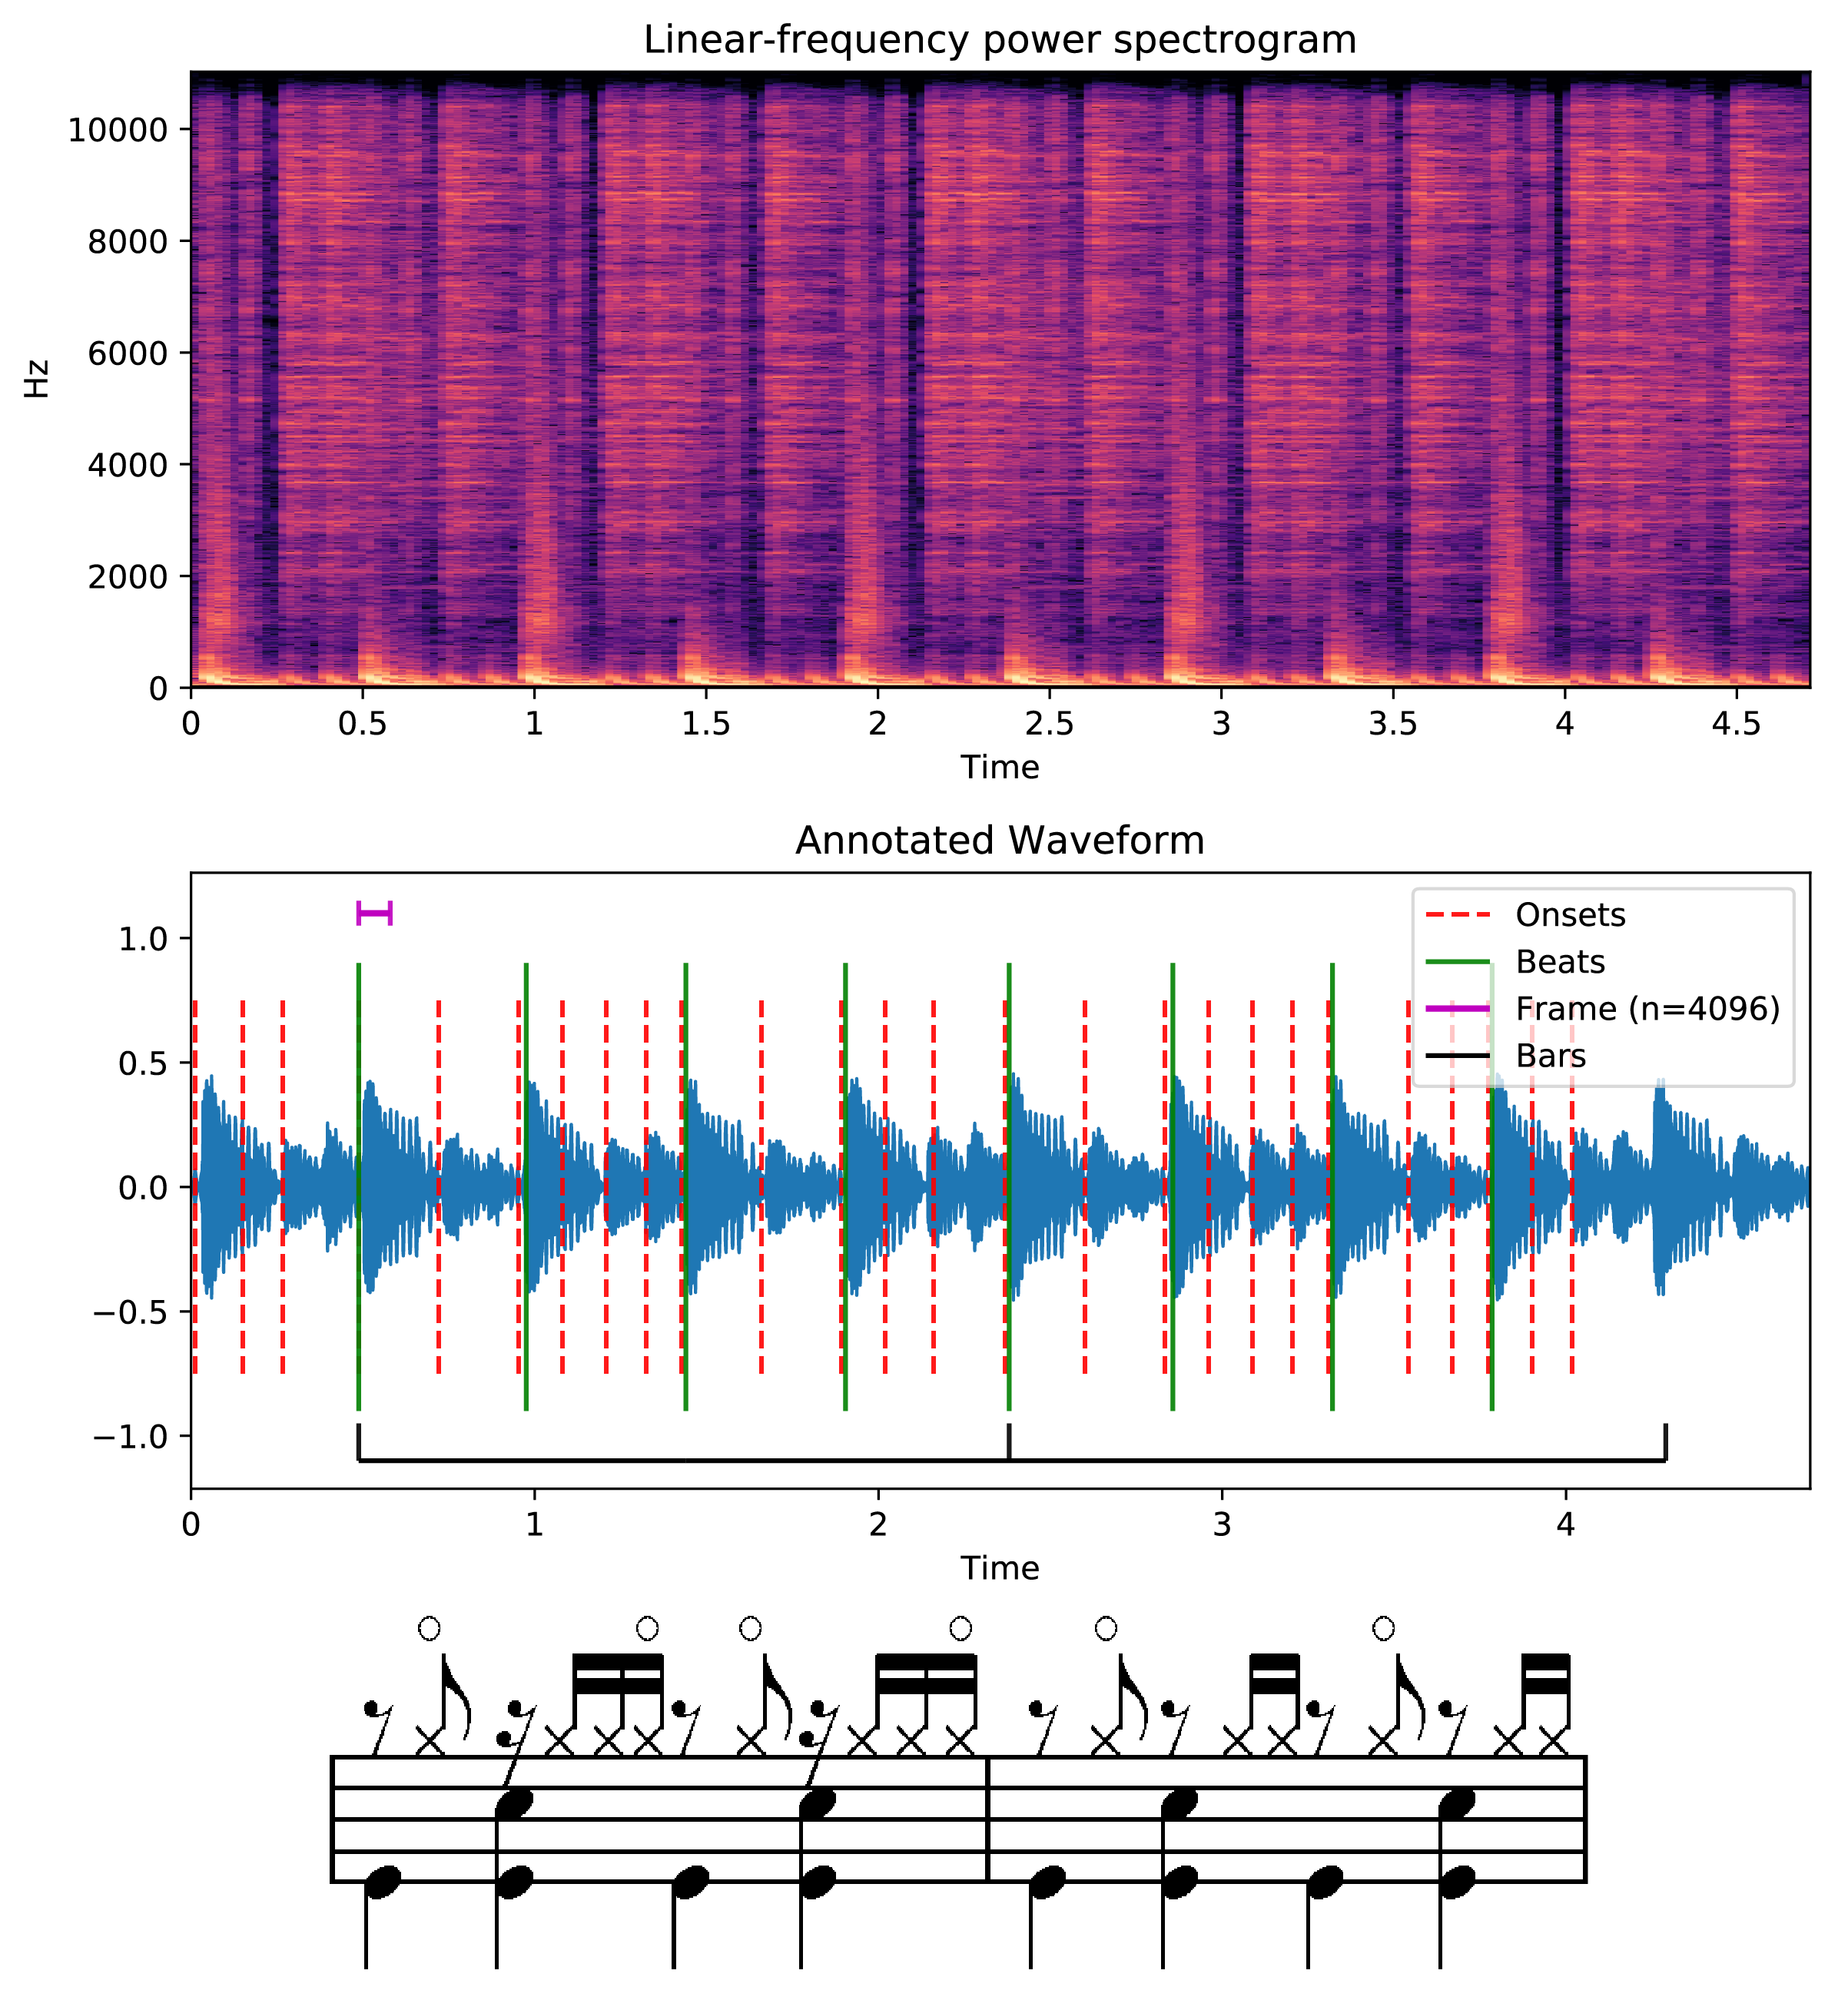
\includegraphics[width=0.75\textwidth]{ch05_pyconcat/figures/unit_plot.png}
	\end{center}
	\caption[Annotated Waveform, Spectrogram and Drum Transcription of ``My Sound'' by Joey Beltram (R\&S Records)]{Annotated Waveform, Spectrogram and (approximate) Drum Transcription of ``My Sound'' by Joey Beltram (R\&S Records)}
	\label{fig:beltram}
\end{figure}

\subsection{Framewise Segmentation}

At the lowest level of unit decomposition is the framewise unit. In granular synthesis many combinations of microsound timescales of typically 20-200 ms are combined to create dense masses of sound “clouds”. Granular synthesis systems typically control the recombination of these sounds in a parametric fashion; the user specifies or manipulates controls determining endmost pitch, length and envelope qualities. As \cite{Schwarz2003} notes, granular synthesis is “rudimentarily data-driven” but can be significantly augmented with pre-feature analysis - what we seek to achieve by performing concatenative synthesis. 

Granular synthesis is generally performed in the time domain, directly moulding and shaping the portions of the waveforms themselves using an amplitude envelope or windowing function based on Gaussian or linear patterns for example \citep{Roads1996, Roads2004}. Another option is to take frame sizes of orders of $2^n$ (512, 1024, 2048 etc). and transform them to the frequency domain using a \acrfull{fft}. Resynthesised signals can be reconstructed later in the time domain later using the \acrfull{ifft} with overlap and add. While not an overly common approach to concatenative synthesis, it has been alluded to by \cite{Kobayashi}, \cite{Puckette2004}, \cite{An2012}, and some practical artistic applications have been summarised by \cite{Schwarz2006b}. The former describes how \acrshort{ifft} synthesis was used in the theatre piece \textit{La Légende des Siècles} (2002) to assemble \acrshort{fft} frames based on a target specification of pitch and energy. Frame-based segmentation and Fourier resynthesis are available as unit scale options in PyConcat, but have only been used and tested sporadically. The drawbacks of operating at this minuscule order of scale is the sheer level of data handling and computation it entails. Furthermore, if the composer is additionally working in the frequency domain they need to take extra care with continuity and phase, something a \acrshort{hmm} unit selection scheme further on would help address. 

%\begin{figure}
%	\begin{center}
%		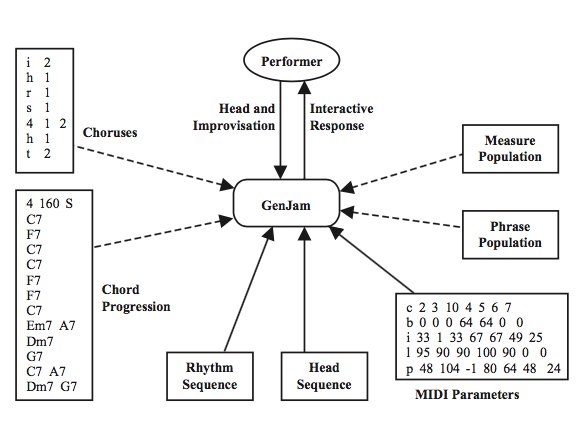
\includegraphics[width=0.8\textwidth]{ch03_symbolic/figures/genjam.png}
%	\end{center}
%	\caption[GenJam Architecture]{GenJam Architecture}
%	\label{fig:genjam}
%\end{figure}

\subsection{Onset Detection for Unit Decomposition}

%If microsonic grains are the de facto unit of scales for granular synthesis then the musical concept of a note with its, is the possibly the equivalent for concatenative synthesis. 
%
%Onset detection methods enables us to build a picture of where musical notes lie in a musical signal by looking for  

\subsubsection{Onset Detection Function}

At the heart of an onset detection algorithm lies the extrapolation of a detection function. The detection function, also referred to as the novelty, change or reduction function is critical in reducing the complete audio signal at its higher sample rate to a lower frequency function of candidate peaks that reveal potential onsets. A detection function tries to detect moments of large change or flux, such that these drastic points of disparity in a signal quality like its energy signify the occurrence of a musical note or percussive transient. Time domain approaches work by taking a frame of audio samples of size $N$, summing the rectified absolute values (as in an envelope follower) or computing the root mean square (RMS) then calculating the 1st-order differential of those values \citep{Laroche2003, Duxbury2002}

More robust methods typically operate in the frequency domain. Critics of time domain methods point to its difficulty in recognising change of events in signals with high energy or noisy background \citep{Grzywczak2014, Eyben2010}. By operating in the frequency domain we can pick up on more information in addition to energy/envelope changes that might prove efficacious in the characterisation of a note event, such as the change of pitch revealed by its shifting spectrogram \citep{Schloss1985, Lerch2012}. Three of the most popular spectral methods include:

\begin{itemize}
\item Spectral Flux: Calculate the distance between two consecutive frames of the magnitude spectrum, using some distance measure such as Euclidean or absolute value.
\begin{equation}
\label{eq:Spectral Flux}	
F(n)=\frac{1}{N}\sum_{k=1}^{\frac{N}{2}-1}\sqrt{(X_{k}(n)-X_{k}(n-1)})^{2}
\end{equation}
\item Complex Flux: \citep{Bello2004} proposed extending the spectral flux method to incorporate phase information in addition to magnitude. By tracking the instantaneous phase of the complex spectrum, the real frequency can be calculated as per the phase vocoder \citep{Roads1996}. If the pitch of a note correspond to a (mostly) steady state frequency, then in theory deviations from the expected phase of a signal should reveal note events of signals where large energy changes are not such prominent indicators.
\item \acrfull{hfc}: Many percussive events are broadband in their frequency content, most notably those involving cymbals or snare sounds. To emphasise the contribution of higher frequencies to the novelty function, frequency bins of the spectrum can be weighted proportionally then summed to produce a framewise \acrshort{hfc} descriptor more tailored for percussive sounds.

\begin{equation}
\label{eq:High Frequency Content}	
F(n)=\frac{1}{N}\sum_{k=1}^{\frac{N}{2}-1}W_{k}|X_{k}(n)|^{2}
\end{equation}

\item Deep Learning Approaches: Reflecting recent trends in the arena of machine learning towards deep learning and application of neural networks, state of the art methods are also delivering some of the most promising results for creating usable novelty functions. \cite{Marolt2002} first proposed using a neural network, trained on a corpus of synthesised piano performances, to detect the presence of onsets in the amplitude envelopes of an \acrshort{iir} filterbank of 22 filtered signals.  \cite{Lacoste2007} proposed using supervised learning of a neural network trained to classify onset or non–onset in frequency representations of the signal, using an \acrshort{stft} and a Constant-Q Transform. Convolutional neural networks, such as those outlined by \cite{Schluter2013, Schluter2014} borrow from object classification tasks in computer vision research to analyse streams of spectrograms. Naturally, and in contrast to the more traditional signal processing methods, the success of supervised learning methods relies greatly on the data used for training.
\end{itemize}

\subsubsection{Thresholding and Peak Picking}
\label{sec:peak_picking}

The novelty functions returned by those methods described in the previous section returns candidate peaks, or in the case of neural network oriented methods, probabilities of candidates that potentially correspond to onset times. To filter out spurious peaks and retain those local maxima, the novelty function needs to be processed through thresholding and application of a peak picking algorithm. 

Fixed thresholding retains only those peaks from the novelty function that exceed a constant threshold value. This works well for program material occupying smaller dynamic ranges, as in highly compressed music or percussive recordings. For material that varies in dynamics over time it is rather crude and inflexible - for such scenarios an adaptive thresholding procedure is preferable. Adaptive thresholding essentially computes another function that gives an instantaneous threshold value for each sample of the novelty function based on some analysis of that very function. Standard methods proposed by
\cite{Bello2005b}, \cite{Dixon2006}, \cite{Bock2012a, Bock2013}, choose a window of time $w$ around the current novelty function sample and derive a rolling average or low pass filtered version of the function and reject peaks below some multiple of that threshold function.

Peak picking, as summarised by \cite{Bock2012a} can finally be applied by constraining the novelty function $F(n)$ to a set of criteria as in:

\begin{equation}
  \label{eq:peak_picking}
  \begin{gathered}
P(n)=max(F(n-w:n+w))\\
P(n)\geq mean(F(n-w:n+w))+\delta\\
n-n_{last}>\beta
  \end{gathered}
\end{equation}

where $n$ is the current frame number, $w$ is a window of frames around $n$, $\delta$ is a threshold multiplier to be applied to the rolling average and $\beta$ is used to reject potential onsets if they occur within a number of frames of a previously detected onset. Naturally, this set of criteria assumes that the source signal already exists in its entirety as in a pre-recorded sound file.

For real-time onset detection it is more challenging as we do not have access to future frames of audio, unless some pre-delay is applied (as is done in look ahead limiters and processors that need some advance information in order to duck the signal). Even if no pre-delay is applied, novelty frames can only be compared to those captured in the past, which at least incurs a delay penalty of $w.N/SR$ milliseconds given frame length $N$ and sample rate $SR$ and frame window $w$.

\subsubsection{Evaluation of State of the Art Onset Detection Algorithms}

Our intention in this thesis is not to reinvent the wheel in basic building blocks for  musical signal processing, thus we propose no new methods for onset detection tasks. We do however, need to evaluate the state of the art methods currently available and compare their suitability for our needs in concatenative synthesis, which is documented in this section.

\paragraph{Datasets}

To evaluate the respective performance of each method, we gathered a number of datasets that are used in the literature and were made available, comprising:

\begin{itemize}
  \item ENST-Drums: Provided by Télécom ParisTech \citep{Gillet2006}, contains an audio-visual annotated dataset of performances by 3 professional drummers using multi-track studio recording in a variety of configurations (single hits, phrases and accompaniments) and a variety of styles including jazz and rock. 
  \item Modal (Musical Onset Dataset And Library): Hand annotated, contains 501 onsets across 71 files containing a mix of mostly monophonic events \citep{Glover2011}
  \item JKU: Contains 321 files with 27,774 total onsets. Compiled from a number of different sources by Sebastian Böck for evaluating his SuperFlux algorithm \citep{Bock2013}. The algorithm was developed especially to handle vibrato, and accordingly the dataset contains a large number of samples that purposely address vibrato, such as samples from opera or Western classical string technique.
\end{itemize}

\paragraph{Algorithms}

Three different exemplar onset detection methods available in the Essentia \citep{Bogdanov2013} and the Madmom \citep{Bock2016} libraries were integrated into our own PyConcat framework and their performances were estimated on the previously described datasets. The specifics of the algorithms themselves are explained as followed:

\begin{itemize}
  \item \textit{Essentia-OnsetRate:} Essentia’s “OnsetRate” algorithm combines the HFC and Complex domain novelty function detection methods. The two functions are multiplied by each other in order to emphasise those frames in agreement with each other. 
  \item \textit{Madmom-Superflux:} Madmom’s implementation of the Superflux algorithm as proposed by Böck et al. (2013). It expands on the spectral flux approach to handle program material that contains soft attacks, and instruments with vibrato tendencies such as strings, winds and the voice, that are difficult to capture using energy differences alone. 
  \item \textit{Madmom-CNN:} Uses a convolutional neural network to detect likelihood of onsets within a frame by frame basis \citep{Schluter2013, Schluter2014}. This algorithm achieved the highest scoring F-Measure and Recall and the second highest scoring Precision of the Onset Detection task as part of MIREX 2016.
\end{itemize}

\paragraph{Procedure}

Onsets were extracted using a batch procedure on all of the audio files with each algorithm using our PyConcat framework. For each audio file a single text file was produced with estimated onset times. These were then compared with the ground truth annotations using the mir\_eval python package, a Python library for evaluating \acrshort{mir} related tasks according to \acrshort{mirex} guidelines \citep{Raffel2014}. An onset is defined as correctly identified if the time annotation is within +/- 50 ms of the ground truth annotation. Errors are categorised as either false positives or false negatives:

\begin{itemize}
  \item \textit{False Negative:} No onset estimation exists for a ground truth annotation
  \item \textit{False Positive:} An onset estimation outside the tolerance window for any ground truth annotation
\end{itemize}

Scores are computed for each file according to the standard information retrieval fractional measures of precision and recall as well as the f-measure, a derived measure that attempts to consolidate both previous measures for easy comparison of overall algorithms’ performance. Borrowing from the definitions provided in the sci-kit learn documentation\footnote{\url{http://scikit-learn.org/stable/auto_examples/model_selection/plot_precision_recall.html}} but adapted for the specific task of onset detection, we can define them as follows (where $T_p$ signifies true positives - correctly identified onset).

\begin{itemize}
  \item \textit{Precision:} the fraction of total estimations that are correct:
\begin{equation}
\label{eq:Precision}	
P=\frac{T_{p}}{T_{p}+F_{p}}
\end{equation}  

  \item \textit{Recall:} the fraction of the total annotations that are correctly retrieved:
\begin{equation}
\label{eq:Precision}	
R=\frac{T_{p}}{T_{p}+F_{n}}
\end{equation}  

  \item \textit{F-Measure:} an aggregate score incorporating both precision and recall, defined as the harmonic mean of both:
\begin{equation}
\label{eq:Precision}	
F_{1}=2*\frac{P*R}{P+R}
\end{equation}  

\end{itemize}

\subsubsection{Results}

Results for all the files from each dataset were collated and statistics computed using mean and standard deviations, as summarised in \tabref{tab:onset_total_results}, while \figref{fig:onset_total_boxplots} provides corresponding box plots visually depicting the distributions. As is evident, the \acrfull{cnn} based onset detector is the highest scoring and most consistent of the onset detectors measured based on overall mean values and the small degree of spread in the box plots. Superflux also delivers excellent results albeit with the introduction of more variance across samples. The combined methods present in Essentia's OnsetRate algorithm performed the most poorly, with the highest degree of spread across all measures.

{\renewcommand{\arraystretch}{1.5}
\begin{table} 
	\begin{centering}
		\begin{tabular}{lllllll}
\tabletop
    Algorithm & \multicolumn{2}{c}{Precision} & \multicolumn{2}{c}{Recall} & \multicolumn{2}{c}{F-Measure}\\
    & Mean & Std. Dev. & Mean & Std. Dev. & Mean & Std. Dev.\\
\tablemid
	\textbf{CNN} & \textbf{0.9208} & \textbf{0.1452} & \textbf{0.9073} & \textbf{0.1603} & \textbf{0.9062} & \textbf{0.1568}\\
	SuperFlux & 0.8719 & 0.1817 & 0.8702 & 0.1849 & 0.8550 & 0.1898\\
	OnsetRate & 0.8412 & 0.2166 & 0.7523 & 0.2287 & 0.7779 & 0.2128\\
\tablebot
		\end{tabular}
		\caption[Onset Detection Algorithm Results]{Onset Detection Algorithm Results}
		\label{tab:onset_total_results}
	\par \end{centering}
\end{table}

\begin{figure}
	\begin{center}
		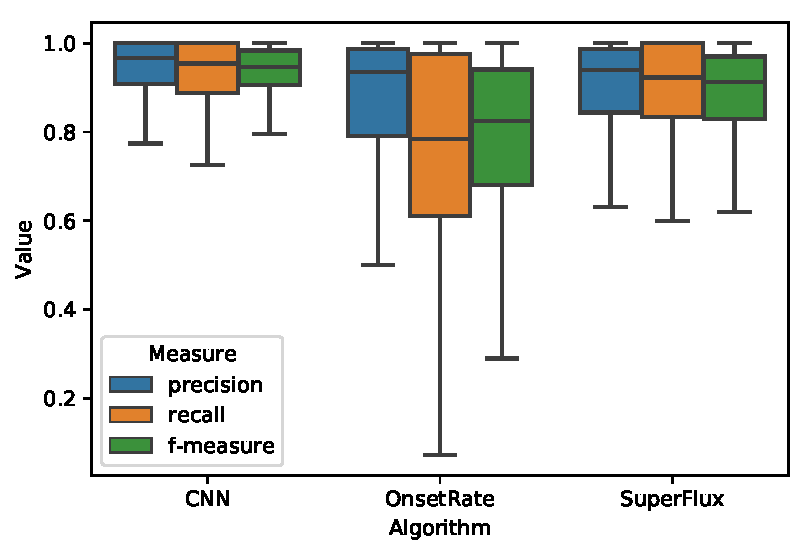
\includegraphics[width=0.75\textwidth]{ch05_pyconcat/figures/onset_total_boxplots.pdf}
	\end{center}
	\caption[Boxplots of Results for each algorithm and measure.]{Boxplots of Results for each algorithm and measure.}
	\label{fig:onset_total_boxplots}
\end{figure}

\tabref{tab:extended_onset_statistics} shows in more detail the statistics for each algorithm separated by the particular datasets evaluated and with the highest precision, recall and F-measure highlighted for each. It is interesting to note that all the algorithms deliver good results on the \acrshort{enst} dataset, which is entirely percussive. Superflux and \acrshort{cnn} perform much better on the \acrshort{jku} dataset on which it is been designed. These algorithms demonstrate their robustness on program material of all types, including sustained vibrato sounds as well as clear transient heavy percussive material.

\begin{sidewaystable}
	\begin{threeparttable} 
		\ra{1.1}
%		\small
		\begin{centering}
			\begin{tabular}{l l l l l l l l l l l}
				\tabletop
Algorithm & Dataset & Onsets & TP    & FP   & FN    & Precision & Recall & F-measure & mean & std \\
				\tablemid			
CNN       & ENST-1  & 8813   & 8057  & 697  & 756   & \textbf{0.921}     & \textbf{0.937}  & \textbf{0.921}     & 2.5  & 5   \\
          & ENST-2  & 10319  & 9738  & 484  & 581   & \textbf{0.945}     & 0.956  & \textbf{0.948}     & 1.6  & 5.4 \\
          & ENST-3  & 11019  & 10154 & 464  & 865   & 0.932     & 0.926  & 0.928     & 2.5  & 5.4 \\
          & JKU     & 25827  & 23293 & 978  & 2534  & \textbf{0.941  }   & \textbf{0.9}    & \textbf{0.916}     & -3.6 & 5.2 \\
          & Modal   & 501    & 418   & 122  & 83    & \textbf{0.774}     & 0.798  & \textbf{0.744}     & -3.9 & 3.2 \\
          \hdashline
Superflux & ENST-1  & 8813   & 7867  & 756  & 946   & 0.911     & 0.931  & 0.915     & -1.4 & 4.9 \\
          & ENST-2  & 10319  & 9553  & 549  & 766   & 0.94      & \textbf{0.957}  & 0.946     & -2.4 & 5.4 \\
          & ENST-3  & 11019  & 10018 & 481  & 1001  & \textbf{0.943 }    & \textbf{0.931}  & \textbf{0.935}     & -1   & 5.3 \\
          & JKU     & 25827  & 20382 & 2820 & 5445  & 0.847     & 0.809  & 0.811     & -5.9 & 5.9 \\
          & Modal   & 501    & 392   & 247  & 109   & 0.714     & \textbf{0.837}  & 0.706     & -4.2 & 3.5 \\
          \hdashline
OnsetRate & ENST-1  & 8813   & 6875  & 560  & 1938  & 0.901     & 0.875  & 0.871     & -5.7 & 7.1 \\
          & ENST-2  & 10319  & 8116  & 447  & 2203  & 0.941     & 0.872  & 0.895     & -6.3 & 7.3 \\
          & ENST-3  & 11019  & 8456  & 572  & 2563  & 0.91      & 0.868  & 0.875     & -5.4 & 7.4 \\
          & JKU     & 25827  & 15736 & 3335 & 10091 & 0.793     & 0.627  & 0.686     & -7.1 & 8.8 \\
          & Modal   & 501    & 333   & 213  & 168   & 0.719     & 0.784  & 0.732     & -4.6 & 4.6 \\
				\tablebot		
			\end{tabular}
			\par \end{centering}		
		\begin{tablenotes}
			\small
%			\item[] ABBREVIATIONS: NA=Not applicable; GD=Group Delay, PDE=Probability Density Estimate
		\end{tablenotes}
			\caption[Extended statistics for each algorithm by dataset]{Extended statistics for each algorithm by dataset}
			\label{tab:extended_onset_statistics}
	\end{threeparttable}
\end{sidewaystable}

The smaller Modal dataset appears to cause the most difficulty for all algorithms, but relaxing the tolerance time-window constraint from its default of 25ms to 50ms (actually the tolerance time used for \acrshort{mirex} tasks) improves the accuracy for all algorithms by a significant factor, suggesting it could be an issue of ground truth annotation style compared with the other datasets.

In terms of running time and overall algorithm performance, \figref{fig:onset_running_times} compares the averaged time and standard error (not visible due to low variance of < 1.0 s between consecutive runs). Recent trends towards deep learning solutions, while displaying promising returns in terms of accuracy over other supervised learning methods, frequently pale in comparison when considering efficiency and running times of the solution. Even with Madmom's built-in facility for distributing computational loads over multiple processors, the \acrshort{cnn} method performs much slower than the two flux based approaches. Quite possibly the scale of the datasets is much larger than typical applications for concatenative synthesis, but the comparative performance of onset detection methods is an important point to consider when we look at real time or at least quasi real time applications in due course.

\begin{figure}
	\begin{center}
		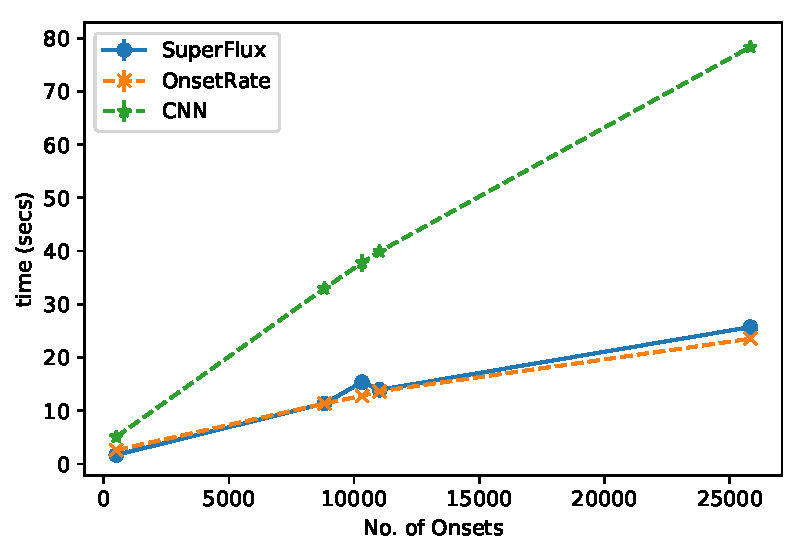
\includegraphics[width=0.75\textwidth]{ch05_pyconcat/figures/onset_running_times.pdf}
	\end{center}
	\caption[Mean and error of the running times of each algorithm over n=10 runs]{Mean and error of the running times of each algorithm over n=10 runs}
	\label{fig:onset_running_times}
\end{figure}

\subsubsection{Beat Tracking and Tempo Extraction}

It seems, from our impression of the literature, that in concatenative synthesis systems the typical unit length is of the onset (or to give it its perceptual equivalent, the note)  \citep{Schwarz2006, Frisson2010, Bernardes2013} - as extrapolated from a suitable onset detection process in the manner previously described. They are reasonably straightforward to compute and represent musically relevant building blocks for producing larger sequences of sounds. But larger musically relevant unit sizes are also a possibility.  Building on top of state of the art techniques in onset detection, \acrshort{mir} researchers are actively trying to coalesce this research with knowledge of tempo and rhythm to pursue algorithms that can perform automatic beat detection within signals.

While an extensive evaluation of state of the art methods in beat detection such as we performed for onset detection is outside of the scope of this thesis, we do summarise some of the key works in this area including their respective \acrshort{mirex} results and expose them as possible unit decomposition options within our own framework. 

\figref{fig:beat_joplin} consolidates various rhythmic concepts from the onset to the bar level and how they relate to the waveform representation and timeline of a typical musical recording. Beats are defined as the perceptual tactus or dominant metrical pulse level that corresponds to where humans are most likely to tap their foot \citep{Jehan2005, Ellis2007a, Stark2009}. A stream of beats implies a certain tempo or \acrlong{bpm} measure of frequency that allow us to understand and compare the speed of musical works, and beat tracking and tempo detection are considered related tasks \citep{McKinney2007}. As \cite{Korzeniowski2014} note, there are many factors in interesting musical recordings that hinder computational facility to determine beats with ease, such as syncopation, hemiola and any other rudimental technique that seeks to thwart regular pulsation. By using tempo estimation and probabilistic prediction of where beats \textit{should} be when they aren't, beat tracking algorithms try to account for these factors. 

\begin{figure}
	\begin{center}
		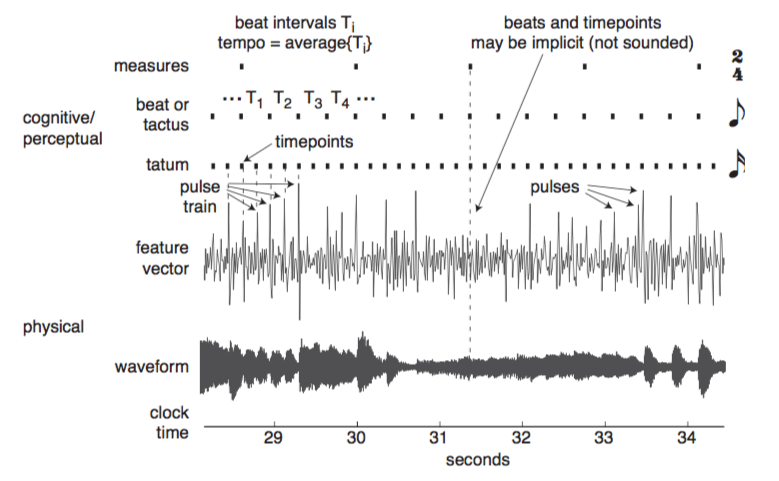
\includegraphics[width=0.9\textwidth]{ch05_pyconcat/figures/joplin.png}
	\end{center}
	\caption[Perceptual and Physical Concepts of Rhythm in a Scott Joplin Ragtime]{Perceptual and Physical Concepts of Rhythm in a Scott Joplin Ragtime. Image from \cite{Sethares2007}}
	\label{fig:beat_joplin}
\end{figure}

\cite{McKinney2007}, provide an excellent summary of the existing state of the art methods at their time of publication, organising the methods by differing implementations of a two stage process. The process consists initially of the \textit{driving} stage, which produces features directly from the signal. This is followed by \textit{periodicity} stage, which outputs estimates of tempo and/or beats based on the analysis of those features \citep{McKinney2007}.

As was emphasised previously, beat tracking studies typically build on onset detection research, as beats essentially represent a perceptual and synchronous subset of onset locations in time. Thus most features\acrshort{hmm} derived for the driving stage consist of applying an onset detection method to produce candidate onset times \citep{Brossier2006, Dixon2006, Ellis2007a, Degara2012, Zapata2014} but not always,   Antonopoulos et al. (2006) for example, use self-similarity of the \acrshort{mfcc} frames as its input. \cite{Degara2012}\footnote{Also one of the beat trackers available in Essentia} build upon their existing offering by integrating multiple input features that include energy flux, spectral flux, difference of mel bands etc. Multiple candidates arising from the various feature inputs are resolved using a method of query by committee and maximum mutual agreement (MaxMA) proposed by the author previously in other work \citep{Zapata2012, Zapata2014}.

The periodicity stage, or where the features are filtered to produce beat locations is where the algorithms deviate the most from each other in terms of approach but many methods in the literature at least start from a probabilistic standpoint. Ellis (2006; 2007) uses onset detection followed by autocorrelation to get an initial estimate of the overall tempo of the track. This information is used by the beat-tracking module to compare the idealised beat times against computing the globally optimised set of beat times using \acrshort{ioi}s and dynamic programming in a manner not so far removed from that proposed by \cite{Alonso2007}. Degara also utilises a \acrshort{hmm}-based algorithm, augmented with an intrinsic framework that models sequences of non-beat states as well as beat states.

A multi-agent system for detecting periodicity has been employed by a number of investigators \citep{Goto2001a, Dixon2007, Oliveira2012}. In the case of Dixon, for instance, an initial tempo hypothesis and potential first beat from an initial set of onsets are assigned to several agents. Predicted beat times are then generated from the initial onset and hypothetic tempo, and onsets falling within a tolerated window of those predictive times are labelled as actual beats. A complex resolution system examines the degree of agreement between agents to decide on the final beat locations.

\paragraph{Current State of the Art and Deep Learning Approaches}

\tabref{tab:beat_tracker_results} shows the F-Measure scores for every algorithm submitted to the 2016 MIREX competition. The datasets under scrutiny include:

\begin{itemize}
  \item \textit{SMC} - 160 30-second excerpts of music in a variety of instrumentation and styles but with a stable tempo. 20\% of the examples contain non-binary meter.
  \item \textit{MAZ} - 367 Chopin Mazurkas with shifting tempos.
  \item \textit{MCK} - 217 tracks of roughly 40s long, with 19 “easy” and 198 “hard” excerpts from Romantic music, film soundtracks, blues, chanson and solo guitar.
\end{itemize}

{\renewcommand{\arraystretch}{1.0}
\begin{table} 
\footnotesize
	\begin{centering}
		\begin{tabular}{lllllll}
\tabletop
	Key & Name & Authors & \multicolumn{4}{l}{F-Measure}\\
		& 	   &		 & SMC & MAZ & MCK & Mean\\
	
				\tablemid			
BK1 & DBNBeatTracker.2016           & S. Böck,          & 56.8313 & 57.5286 & 63.6093 & 59.3231 \\
    &                               & F. Krebs          &         &         &         &         \\
BK3 & DBNDownBeatTracker            & S. Böck,          & 52.8343 & 73.8911 & 62.5299 & 63.0851 \\
    &                               & F Korzeniowski    &         &         &         &         \\
BK2 & CRFBeatDetector.2016  			& S Böck,           & 52.3142 & 55.1651 & 62.7315 & 56.7369 \\
    &         						& F Krebs           &         &         &         &         \\
SB9 & BeatRoot Vamp Plugin          & S. Böck           & 52.097  & 58.9357 & 63.8961 & 58.3096 \\
SB8 & QM Tempo Tracker              & S. Böck           & 49.8366 & 52.2792 & 63.8436 & 55.3198 \\
JZ1 & MultifeatureBT-Inf-7odf-Repet & J. R. Zapata      & 36.8192 & 50.63   & 52.6104 & 46.6865 \\
JZ2 & MultifeatureBT-Reg-7odf-Repet & J. R. Zapata      & 36.4073 & 47.874  & 53.2314 & 45.8376 \\
CD3 & QM Tempo Tracker              & C. Cannam,        & 33.663  & 49.6229 & 52.8758 & 45.3872 \\
    &                               & M. Davies         &         &         &         &         \\
CD2 & BeatRoot Vamp Plugin          & C.Cannam & 30.34  & 41.5218 & 52.6579 & 41.5066\\
 	&           					& S.Dixon 			&    &  &  & \\
\tablebot
		\end{tabular}
		\caption[Mirex 2016 Beat Tracking Results]{Mirex 2016 Beat Tracking Results}
		\label{tab:beat_tracker_results}
	\par \end{centering}
\end{table}

%\begin{sidewaystable}
%	\begin{threeparttable} 
%		\ra{1.1}
%		\begin{centering}
%			\begin{tabular}{lllllll}
%				\tabletop
%
%				\tablebot		
%			\end{tabular}
%			\par \end{centering}		
%		\begin{tablenotes}
%			\small
%%			\item[] ABBREVIATIONS: NA=Not applicable; GD=Group Delay, PDE=Probability Density Estimate
%		\end{tablenotes}
%			\caption[Extended statistics for each algorithm by dataset]{Extended statistics for each algorithm by dataset}
%			\label{tab:extended_onset_statistics}
%	\end{threeparttable}
%\end{sidewaystable}


Beat tracking is a significantly more complex task compared to onset detection, and evidently the results reflect this. Ranges of accuracy vary greatly across the different datasets and while no single algorithm achieves the highest F-Measure, at least Böck and Korzeniowski’s DBNDownBeatTracker manage to attain the highest mean performance. Once again we see the headway deep learning based methods are making in all manner of pattern recognition and machine learning tasks, as this method relies on a recurrent neural network armed with a bank of resonant comb filters. 

\subsection{Future Directions - Mixing and Source Separation}

Most concatenative synthesis systems we have studied (including those techniques we propose) tend to consider the concatenation process in purely horizontal and temporally inclined terms.  Naturally, it is pertinent to question whether the same process can be applied systematically in the vertical dimension characterised by the frequency spectrum. Or in more simpler terms - can we stack units on top of each other systematically in addition to chaining them in sequence? While not the focus of this thesis (but certainly a promising avenue for further study), we briefly summarise relevant topics of interest and  techniques that are or can be used.

\subsubsection{Vertical Selection with Mixture Models}

\cite{Hoffman2009} have outlined a system that seeks to recreate the target \textit{spectrum} by, as Coleman describes it \citeyearpar{Coleman2010}, \textit{superimposing} (using convolution) a series of spectra from a corpus. To reduce the complexity associated with high dimensionality search space a \acrfull{mcmc} is applied. 

In a version of AudioGuide by Hackbarth \citep{Hackbarth2013}, they also outline the system's facility for enabling ``layered sounds'' and ``vertically stratified complexes'' based on formulas developed by \cite{Tardieu2008} and Carpentier for a prior system in the OpenMusic environment called Orchidée or Automatic Orchestration Tool \cite{Carpentier2010}. The goal of their work is to transfer some of the principles of traditional orchestration (combining and arranging for instruments to create desired blends of timbre) to the realm of computer music by allowing prediction of mixtures as well as concatenations to match a target specification of a sound.

Hackbarth \citep{Hackbarth2010} describes the derived ``Subtractive Spectral Algorithm'' for superimposition. When an appropriate unit is selected from the corpus as a candidate match for the target its time-varying mel-amplitudes are subtracted from the target sound and a `residual' target spectrum remains. The unit selection procedure is performed repeatedly until it halts when the residual target spectrum energy falls below a certain threshold. The resulting units are then mixed together additively. A visual depiction of this over several mixtures can be see in \figref{fig:spectrum_subtraction}. Clearly the algorithm tends towards selection of louder units initially, with gradually softer ones emerging as the subtracted target energy diminishes. 

\citep{Coleman2015} invokes the term ``mixtures'' to describe concatenative synthesis problems where the corpus might not have all the features to effectively simulate a target but a carefully selected combination of them might, and uses the analogy of several single notes combining to form a chord, except the synthesis engine would use a weighted combination of superimposed frames mixed together.

\begin{figure}
	\begin{center}
		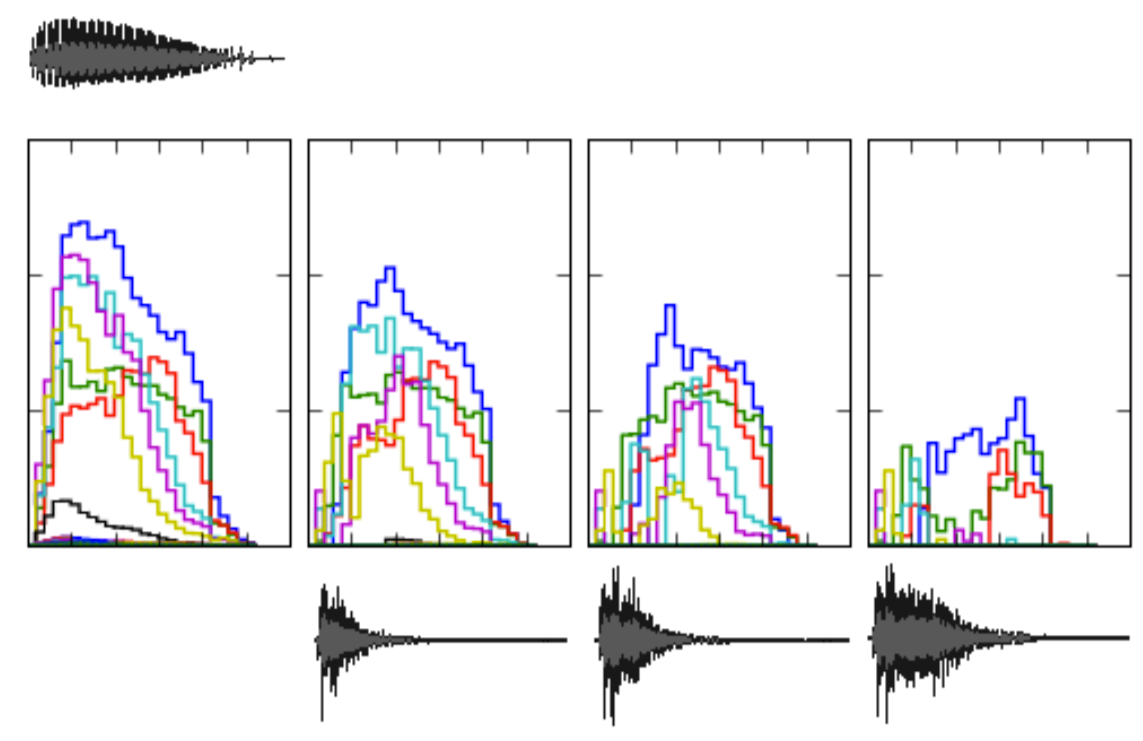
\includegraphics[width=0.75\textwidth]{ch05_pyconcat/figures/spectrum_subtraction}
	\end{center}
	\caption[Spectral Subtraction Algorithm in AudioGuide]{Visual depiction of spectral subtraction algorithm in AudioGuide. Image from \cite{Hackbarth2010}.}
	\label{fig:spectrum_subtraction}
\end{figure} 

\subsubsection{Vertical Segmentation with Source Separation}

As we highlighted previously in the case of the missing fundamental frequency, our auditory system is remarkable in its processing ability and inference engine. More remarkably,  perhaps, is its innate capacity for on the fly separation of real-time audio signals at will, or to give it its technical term, blind source separation. In pyschoacoustic auditory scene analysis research \citep{Bregman1994}, source separation is illustrated usually in terms of the ``Cocktail Party Effect'': how is a human, at a social event, able to separate voices from background noise and home in on particular conversations? In musical source separation this is even more elusive - consider picking out individual instruments in an orchestral passage, especially when, as \cite{Miron2017a} stresses, sources are likely to be correlated in time and frequency. Computational auditory scene analysis seeks to replicate this extraordinary human processing ability through digital signal processing means \citep{Wang2006}.

Initial efforts in computational source separation often involved matrix decomposition methods such as non-negative matrix factorisation as demonstrated in the work of 
\cite{Fitz2004}. Fitzgerald's initial focus was on automatic drum transcription via source separation but later gained wider recognition with some some successful demixing and upmixing from mono to stereo of recovered archive Beach Boys recordings \citep{Fitz2004}. More recent state of the art approaches are once again successfully exploiting deep learning methods trained on large sets of musical data in genres like Western classical \citep{Miron2017a, Miron2017}.

Just as a concatenative synthesis system will use onset detection to split larger sound files into smaller units along the time domain, source separation opens up the possibility of theoretically segmenting complex sounds in the frequency domain according to instrument (all depending of course on the material to be separated and the models upon which the system has been trained).

This we can envisage as particularly useful in concatenative synthesis of drum rhythms. Perhaps a producer might want to decompose a number of kits into their constituent parts and mix and match with sounds from other sources. Mixing electronic drum sounds generated by a drum machine with naturally recorded acoustic drum sounds is a common strategy in dance music and source separation could prove invaluable here.

\section{Describing Sounds with Features}

\subsection{Temporal Descriptors}

\subsubsection{Intensity and Loudness}

Physically speaking, sound is a medium transporting mechanical energy via waves. In recorded media, analog or digital signals are converted to electrical and magnetic energy that push speakers backwards and forwards in a manner analogous to the original waveform captured.

Digital signals are essentially a series of amplitude values sampled at a particular sampling frequency. Taking the absolute value at an instantaneous sample point or the maximum absolute value over a window of samples gives us the peak amplitude. Unless the peak amplitude occurs frequently, in itself it is not a very useful indicator of the overall amplitude of the signal, thus the \acrfull{rms} is computed on the window of samples to get a better statistic of the general power of the signal \citep{Puckette2006}:

\begin{equation}
\label{eq:rms}	
A_{RMS}\{x[n]\} = \sqrt{\frac{1}{N}(x[1]^2, x[2]^2,..., x[N]^2}
\end{equation}

where $N$ is the length of the discrete time signal $x$ and $x[n]$ are the individual samples. Most other works we have encountered related to concatenative synthesis use \acrshort{rms} as their principal loudness descriptor, particularly \cite{Sturm2004} and \cite{Bernardes2013}, but \cite{Jehan2005} computes his loudness descriptor from energy in the frequency domain.

Human perceptual response to increments in amplitude is intrinsically logarithmic, thus to aid relative comparisons and metering purposes amplitude values are often computed as a ratio of some reference value and reported using the \acrfull{db} scale, as Puckette \citeyearpar{Puckette2006} indicates. 

\begin{equation}
\label{eq:decibel}	
d = 20.\log_{10}{\frac{a}{a_{0}}}
\end{equation}

\begin{figure}
	\begin{center}
		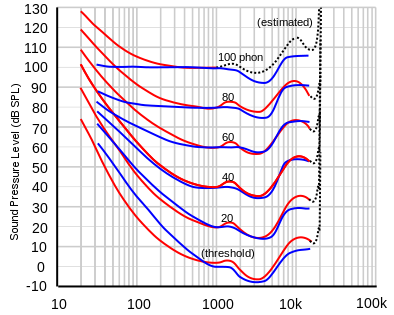
\includegraphics[width=0.75\textwidth]{ch05_pyconcat/figures/fletcher_munson.png}
	\end{center}
	\caption[Fletcher-Munson Curves]{Equal-loundness curves in red with ISO revisions in blue. Image from Wikipedia.}
	\label{fig:fletcher}
\end{figure}

Intensity, power, energy etc. are all \textit{objective} physical concepts. We use the term \textit{loudness} to describe the subjective human perceptive experience that we feel when exposed to intensity of sound. As \cite{Lerch2012} points out, the decibel is neither a true indicator of loudness because "equal-sized steps on the decibel scale are not perceived as equal-sized loudness steps by human listeners", or as \cite{Stevens1955} puts it more succinctly: "equal steps do not sound like equal steps".

Perceived loudness depends on many factors, and, as the long established  Fletcher-Munson equal-loudness contours reveal, it is heavily skewed by frequency. Introduced in the 1930s \citep{Fletcher1933}, subsequently revised as an ISO standard in \cite{countours}, this set of curves (\figref{fig:fletcher}), produced using listening tests, estimates frequency versus sound intensity pressure level where listeners perceive loudness to be roughly equal. To make matters worse, these curves change according to overall intensity, such that at  the difference is more pronounced between frequency ranges at low intensities, while gradually flattening out as intensity increases.

Luckily, more pyscho-acoustically aware measures that take into account such subtleties and phenomena are implemented and available as content analysis features. The \acrfull{ebu}, for example, proposes the \acrshort{ebu} R 128 metering standard in an effort to enforce normalisation consistency across differing programme material in broadcasts\footnote{And combat au-fait advertising and music producers exploiting dynamic range compression to make their products stand out from others.} \citep{ebu, Lerch2012}. It consists of a perceptually tuned K-weighting filter followed by mean square power estimated at momentary, short-term and longer-term intervals.

We are using content analysis mainly for our unit selection algorithm to compute similarity between feature vectors so advanced metering standards like the \acrshort{ebu} R 128 are a bit overkill for our purposes. Another, more basic loudness descriptor available in Essentia's library implements Stevens' Power Law. Stevens' Power Law arose out of efforts to improve on the Weber-Fechner pyschophysics laws that relate changes in physical stimuli with perceptual response to those changes \citep{Stevens1975, Reiss2001}. IT is elegant:

\begin{equation}
\label{eq:stevens}
S(i)=k.i^{n}
\end{equation}

where $S$ is the sensation (perceived magnitude), $i$ is the intensity, $k$ is a unit dependent constant and $n$ is an exponent that depends on the stimulus. Through many perceptual experiments, Stevens produced exponents for a wide variety of physical stimuli, ranging from brightness of light to taste when exposed to sucrose or salt, for example. In the case of loudness, that exponent is estimated at 0.67 \citep{Stevens1975}, and in Essentia it is implemented as the signal energy \eqref{eq:energy} raised to that exponent \eqref{eq:stevens_loudness}.

\begin{equation}
\label{eq:energy}
E\{x[n]\}= \sum_{n=-\infty}^{n=\infty}|x[n]|^{2}
\end{equation}

\begin{equation}
\label{eq:stevens_loudness}
L\{x[n]\}= E\{x[n]\}^{0.67}
\end{equation}

We use the Stevens' Law based descriptor in our systems as it provides (in our view) an acceptable trade off between ease of integration, and grounding in some awareness of perceptual theory. Loudness is a scalar feature, and one of two features we compute solely in the time domain. It is an extremely important quantity that is essential in ensuring that units selected match not only the overall naturalness and dynamics of the target sound, but also remain consistent over the continuous trajectory of the sequence subsequent to concatenation. 

\subsubsection{Log-Attack Time}

The evolution of the energy in a sound is frequently described in terms of its attack, decay, sustain and release envelope \citep{Peeters2004b, Kim2006, Brossier2004a} and is a central facet of modular and digital sound synthesis \citep{Russ2004}. 

Technically it is resolved by taking the logarithm of the time taken from $t0$ to $t1$, where $t0$ is some initial energy percentage of the envelope, while $t1$ is some maximal percentage of the envelope, indicating the end of the attack and the start of the decay or sustain portion (\eqnref{eq:lat}).

\begin{equation}
\label{eq:lat}
lat = log(t1-t0)
\end{equation}

Why do we take the logarithm? Well, just like other perceptual responses to physical stimuli  studies have found higher degrees of correlation in studies examining timbre discrimination when the logarithm is applied.\citep{McAdams1995, McAdams1999, Agres2016}. The log attack time is obviously very useful for discriminating sounds that have distinctive attack profiles \citep{Herrera-Boyer2003}, such as the flute versus a snare drum for example, so naturally this feature makes more sense for ``one-shot'' instrumental classification versus excerpts of recordings for the purposes of genre detection.

\subsection{Spectral and Timbral Descriptors}

Timbre is an extremely complex and elusive aspect of sound for a very simple reason: it is a quality that is likely an emergent property, with indeterminate dimensionality \citep{Elliott2013, Siedenburg2017} or even dimensionality exclusive to a particular timbre \citep{Krumhansl1989}. A typical definition usually follows along the lines of that issued by the Acoustical Society of America:

\blockcquote[]{ansi}{``\textit{That attribute of auditory sensation which enables a listener to judge that two nonidentical sounds, similarly presented and having the same loudness and pitch, are dissimilar}''} 

An elegant distillation undoubtably, but other researchers point out \citep{Siedenburg2017} there is difficulty in these so-called ``wastebasket'' reductionist attempts that leave us none the wiser:

\blockcquote[]{McAdams1979}{``\textit{timbre tends to be the the psychoacoustician's multidimensional waste-basket category for everything that cannot be labeled pitch or loudness.}''} 

\blockcquote[]{Bregman1994}{``\textit{This is, of course, no definition at all. [...] The problem with timbre is that it is the name for an ill-defined wastebasket category. [...] I think the definition [...] should be this: ‘We do not know how to define timbre, but it is not loudness and it is not pitch.’ [...] What we need is a better vocabulary concerning timbre.''}}

\subsubsection{Fourier Analysis (and Synthesis)}

A working knowledge of Fourier analysis and awareness of the first point does give a starting point for many systems that deal with timbre. Fourier's theorem says that any sound in the time domain can be transformed to a sum of sinusoid functions and associated amplitudes in the frequency domain or spectrum \citep{Roads1996}. Overlapping frames of samples taken from a longer signal can be multiplied by a suitable window function, giving a better indication of the evolution of the sound over time, in what is known as a the \acrshort{stft} or spectrogram (if observing just the magnitude) \citep{Collins2010}(\eqnref{eq:stft}).

\begin{equation}
\label{eq:stft}
X[n,k] = \sum_{n=0}^{N-1}\{w[n]x[mH+n]e^{-j2\pi kn/N}\}
\end{equation}

where $w[n]$ is a window function, $H$ is a hopsize, $m$ is the hop number and $k$ is the frequency bin number. If two sounds have the same pitch and loudness - or objectively speaking, the same \textit{perceived} fundamental frequency and amplitude - then perhaps examining the spectrogram should give us a better indication as to what discriminates the two. Examining different sounds using Fourier analysis shows us how different sounds are made up of spectrograms that not only have different magnitudes at different peaks, but also these magnitudes and peaks can evolve over time according to unique envelopes. These peaks in the spectrum are known as partials. When examining musical signals in a spectrum, we call the first partial that is at the lowest frequency in the signal as the fundamental frequency or first harmonic\footnote{Though the human cortex has the extraordinary ability to ``fill in'' a missing fundamental (or \textit{pitch of residue} \citep{Weihs2009}) for a complex harmonic tone even when absent.}. Any partial above this fundamental frequency that is related to the fundamental by an integer ratio is furthermore labelled as the second, third, fourth harmonic and so on, forming the harmonic series \citep{Puckette2006}.

Fourier theory also gives us a constructionist framework for additive synthesis of sounds - by carefully mixing parameters of a bank of sinusoids we can arrive at more complex sounds and even try to mimic some of those found via analysis. But additive synthesis gets very complicated very quickly. Besides having to keep track of large sets of parameters, computing huge banks of sinusoid functions concurrently is computationally expensive. Typical analog and digital synthesisers in the music producer's arsenal approach the problem from the other direction. Complex signals such as squares, sawtooths, or certain shapes drawn in a wavetable are filtered and sculpted to arrive at the desired sound in a process known as \textit{subtractive} synthesis. \acrfull{fm} synthesis also famously uses parametric control of a carrier signal's frequency modulated by a modulation frequency to produce a wide palette of sounds but its minimal set of parameters can prove notoriously complex and difficult in trying to fathom a preconceived sound. 
 
Getting back to spectral and timbral analysis\footnote{It's also worth mentioning spectralism here, a post-Serialist movement in European composition that ran tandem to the burgeoning minimalism across the Atlantic. At \acrshort{ircam}, Gérard Grisey and Tristan Murial harnessed computational analysis of spectra to inspire dense scores on chamber works such as \textit{Les espaces acoustiques} and \textit{Gondwanda} \citep{ross2007rest, Harvey2000}}, the Fourier transform and its spectrogram is a central concept in musical signal processing, and while usually not employed directly as a raw feature in itself, it forms the basis for numerous other algorithms (recall its role in flux based onset detection) and descriptors in \acrshort{mir} literature and systematic practice which we will now turn to. 

\subsubsection{Spectral Centroid}

The spectral centroid gives a scalar value indication of the ``centre of gravity'' in the spectrum of the signal, and as such is computed as the weighted mean of the spectral bin frequencies, with the magnitudes acting as weights (\eqnref{eq:centroid}).

\begin{equation}
\label{eq:centroid}	
c = \frac{\sum_{i=1}^{N}f(i)m(i)}{\sum_{i=1}^{N}m(i)}
\end{equation}

where $f(i)$ is the centre frequency of bin $i$, and $m(i)$ is its associated magnitude. It is considered a robust and reliable indicator of the perceptual ``brightness'' of a sound \citep{Schubert2004}, and is utilised in a variety of systems that classify sounds. In \figref{fig:spectral_features} we can see three different impressions of a drum pattern (programmed in Ableton with a TR-909 preset). The top image shows the ``symbolic'' step pattern notation as would be used in a \acrshort{midi}-based production environment such as Ableton. The middle image the shows the rendered waveform (or time-domain representation) of the drum pattern. Finally in the bottom image the log frequency/ power spectrum shows the frequency domain impression of the signal. Overlaid on the spectrogram, in green, is the spectral centroid computed for every frame of the spectrogram. As we can see the centroid follows the envelope shape of the centre of energy for the spectral evolution of the signal.

\begin{figure}
	\begin{center}
		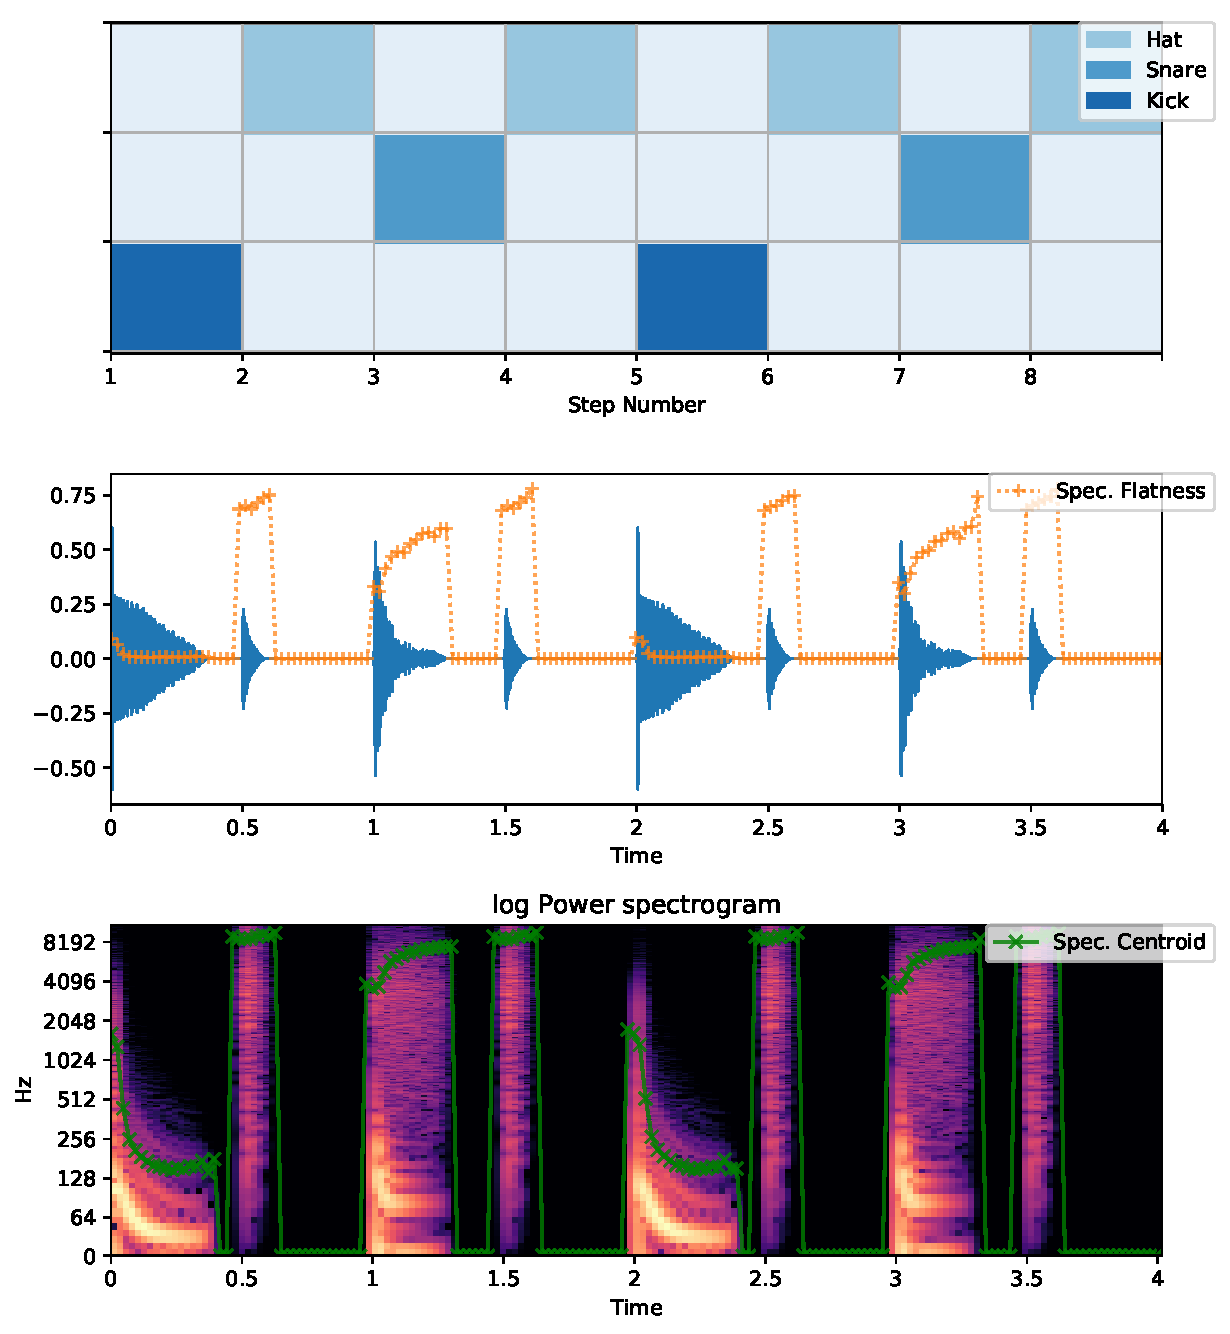
\includegraphics[width=0.85\textwidth]{ch05_pyconcat/figures/spectral_features.pdf}
	\end{center}
	\caption[Spectral features of a drum pattern]{Symbolic grid representation of drum pattern (top). Waveform with spectral flatness (middle). Audio spectrogram with spectral centroid (bottom).}
	\label{fig:spectral_features}
\end{figure}

\subsubsection{Spectral Flatness}

Another feature computed on the spectral profile at each frame is the spectral flatness. The spectral flatness or ``Wiener entropy'' gives an indication of how peaky or flat the spectrum is. Peaky spectra tend towards 0.0 and are indication of more harmonic or tonal sounds while a perfectly flat spectrum of 1.0 indicates stochastic noise. Mathematically it is defined as the geometric mean of the bin amplitudes of the spectrum divided by the arithmetic mean of the same bin amplitudes (\eqnref{eq:flatness}). 

\begin{equation}
\label{eq:flatness}	
f=\frac{\sqrt[N]{\prod_{n=0}^{N-1}X(n)}}{\frac{\sum_{n=0}^{N-1}X(n))}{N}}
\end{equation}

In \figref{fig:spectral_features} in the middle image we observe the spectral flatness has been plotted against the waveform view. Since the range bounds of spectral flatness fall between 0.0 and 1.0 this makes more sense than trying to normalise it into a range that can be plotted easily against the spectrogram. In any case, it can be clearly seen how the flatness function, while reasonably correlated with spectral centroid overall, deviates and approaches the origin for the kick timbre. While percussive sounds are generally considered to be less ``tonal'' overall compared to their non-percussive counterpoints, low frequency membranes such as kick drums and tom-toms do exhibit more discernible pitch compared to the clearly more broadband profiles in the snare and hi-hat, and this is evident simply by looking directly at the relevant time points in the spectrogram. Indeed, typical recipes for synthesising electronic kick drums (such as those found in Roland gear) often suggest combining a sine wave with an envelope controlling a sharp decay in frequency with some short impulse of filtered noise (to create a percussive ``click'') \citep{Risset1999, Reid2002}.

\begin{figure}
	\begin{center}
		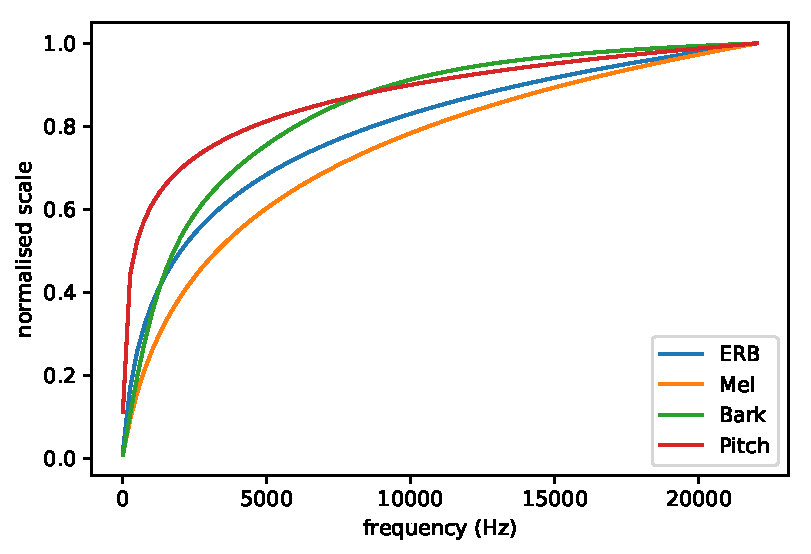
\includegraphics[width=0.8\textwidth]{ch05_pyconcat/figures/scale.pdf}
	\end{center}
	\caption[Perceptual Scales for Audible Range]{Different perceptual scales (normalised) for the audible frequency range}
	\label{fig:perceptual_scales}
\end{figure}


\subsubsection{Cepstrum Analysis}

Effective analysis of complex timbres in musical and natural signals typical employ derived features that exploit some understanding of human perception. The human ear is typically believed to respond to the dynamic limits of 0-120dB and frequency ranges of roughly 20Hz - 20kHz\footnote{Thanks to many years of ignoring advice on earplugs, I strain to hear anything above 14kHz!}\footnote{A famous anecdote recounted by revered console designer Rupert Neve claims that Beatles engineer Geoff Emerick discovered an anomaly in a desk that was attributed to an oscillation at 54kHz \citep{Winer2012}, but later they concede that this was probably due to suboscillatory spillage into the audible range.}. But as we know, human sensation to stimuli is not linear - we don't perceive phenomena in the same way physical measurements are made. The upshot of this is that important information "spreads out" at higher frequencies compared to the more compact resolution of the lower bands.

Pitch is the perceptual description we give to the way our brains organise frequency for the purposes of music. If a tone is perceived to have a pitch at a particular frequency, doubling the frequency of that tone is perceived as the same pitch except one \textit{octave} unit higher.

Depending on when (what era) and where (what culture) you were born in the world how that octave is divided up can be very different (take for example, just intonation or Indian art music). Assuming the chromatic scale based on equal temperament tuning, its octave is divided into 12 semitones using the following formula:

\begin{equation}
\label{eq:High Frequency Content}	
p = 69 + 12 * \log_2(\frac{f}{440})
\end{equation}

What is essentially happening here is a type of frequency warping - compressing sound frequency onto a smaller, perceptual scale that is more tuned for human perception and cognition. In fact, there are other frequency warping formula in the literature that serve to warp frequency according to some conceptually pyschoacoustical or perceptual scale. \figref{fig:perceptual_scales} shows a number of perceptual scales and their normalised output with frequency in Hz as input, notice how they all exhibit a sharp rise that flattens out as it approaches the upper bounds of human response to frequency.

Cepstrum analysis has been one of the most dominating analysis techniques in speech processing for a long time. The word cepstrum itself rearranges the first four letters of the word spectrum, and has been described variously as a type of ``spectrum of a spectrum''. Its usage within speech analysis stems from the fact that it allows to separate the two dominant spectra of a vocal sound - the initial glottal impulse excitation and the slower resonance of the vocal tract \citep{Roads1996, Kim2006}.

To compute cepstrum is comparatively straightforward. The \acrshort{fft} of the signal is taken as normal. The magnitude is retained and the log magnitude spectrum is computed. Finally, the inverse \acrshort{fft} (\acrshort{ifft}) is applied to the log magnitude spectrum. However, normally some frequency warping formula is applied to compress the spectrum in some pyschoacoustic and perceptually motivated manner, and it is here we derive the family of features that include \acrfull{mfcc}, \acrfull{bfcc} and \acrshort{gfcc} (Gammatone Frequency Cepstrum Coefficients warped according to Equivalent Rectangular Bands \citep{Shao2009}). \figref{fig:bfcc_mfcc_gfcc_compared} shows the computed coefficients and the ranges of these features side by side for visual comparison.

\paragraph{MFCCs}

MFCCs are the most common flavour of cepstrum analysis \citep{Kim2006}. \acrshort{mfcc}s use a Mel-spaced filterbank to convert the spectrum to energy in Mels (\figref{fig:perceptual_scales}). The Mel scale, based on perceptual experiments performed by \cite{Stevens1937}, provides a mapping from frequency to Mel pitches that listeners have deemed equal to each other in distance, in a manner similar to the equal-loudness contours previously. While not visible in the normalised representation in \figref{fig:perceptual_scales}, as \cite{Kim2006} notes, the Mel scale and frequency are actually linearly correspondent up until around $500Hz$, at which point it begins to space out across the upper range.

The formula for converting frequency in Hz to Mel pitches is given by:

  \begin{equation}
	\label{eq:mel}	
	m = 2595\log_10 (1+\frac{f}{700})
	\end{equation}
	
\begin{figure}
	\begin{center}
		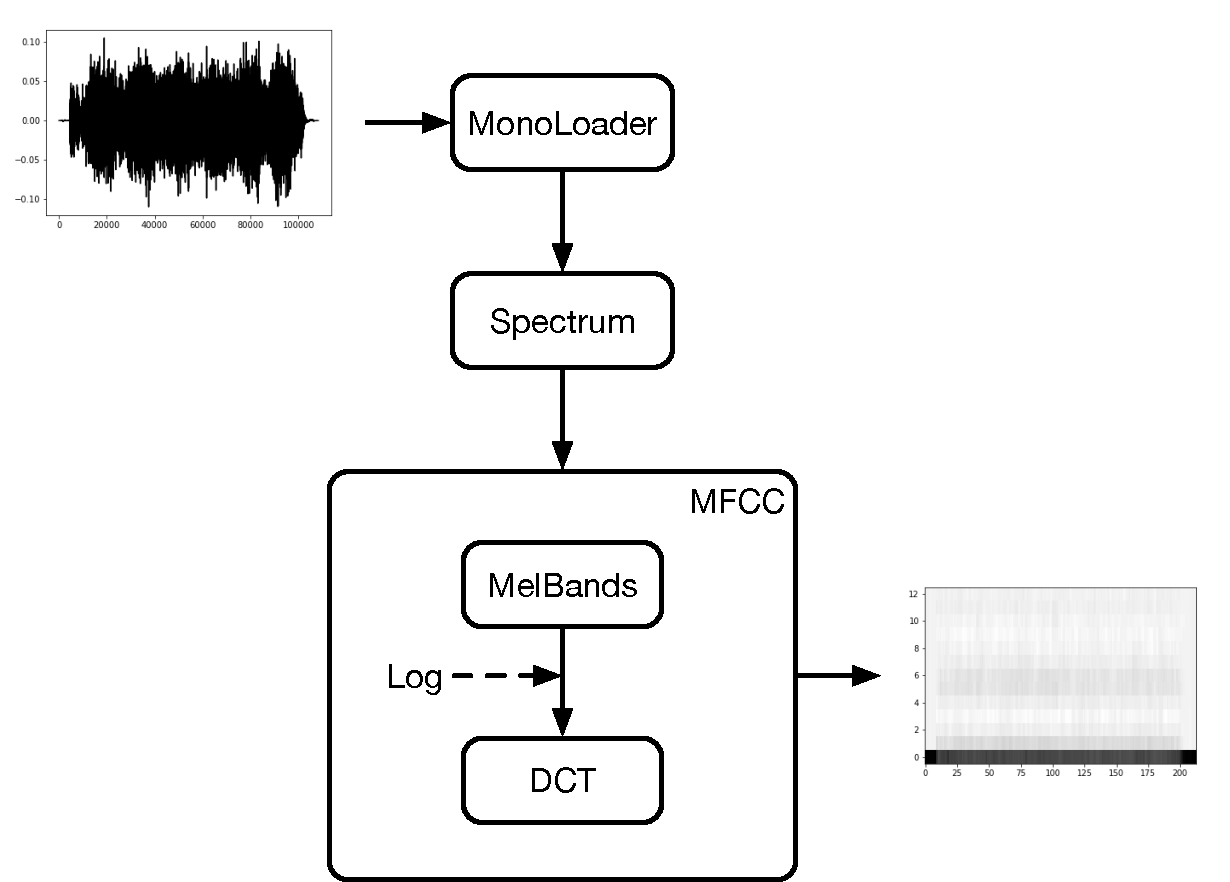
\includegraphics[width=0.9\textwidth]{ch05_pyconcat/figures/mfcc_diagram.pdf}
	\end{center}
	\caption[Signal Flow and Essentia Algorithm Graph for MFCC Computation ]{Signal Flow and Essentia Algorithm Graph for \acrshort{mfcc} Computation }
	\label{fig:mfcc_diagram}
\end{figure}	

To compute the \acrshort{mfcc}s the following steps are taken \citep{Logan2000, Lyons2015}:

\begin{enumerate}
  \item Perform the STFT as given by \eqnref{eq:stft}.
  \item Get the magnitude given by $M(n) = |X(n)|$.
  \item Get the log magnitude given by $L(n) = log(M(n))$.
  \item Warp the log-magnitude spectrum to the Mel scale using 40 triangular filters according to \eqref{eq:mel}.
  \item Finally take the Discrete Cosine Transform \eqref{eq:dct} of the Mel-Frequency log spectrum to obtain the 40 MFC coefficients.
  \begin{equation}
	\label{eq:dct}	
	X_k=\sum_{n=0}^{N-1}x_n cos [\frac{\pi}{N}(n+\frac{1}{2})k]
	\end{equation}
\end{enumerate}

\figref{fig:mfcc_diagram} shows how MFCC extraction is performed in the Essentia environment, showing the signal flow through the various stages, conceptually encapsulated as algorithms. Essentia processes data in a graph-based network, not unlike signal flow languages such as \acrshort{pd} and Max; objects (or algorithms) are connected virtually to each other, and more complex algorithms (composite algorithms) can be assembled by combining other algorithms with processing routines. This is actually the case with the \acrshort{mfcc} algorithm, which as can be seen in the figure receives a spectrum, uses the MelBands algorithm to filter the spectrum, computes the logarithm then finally outputs the \acrshort{mfcc} result from the \acrshort{dct} algorithm. 

\begin{sidewaysfigure}
	\begin{center}
		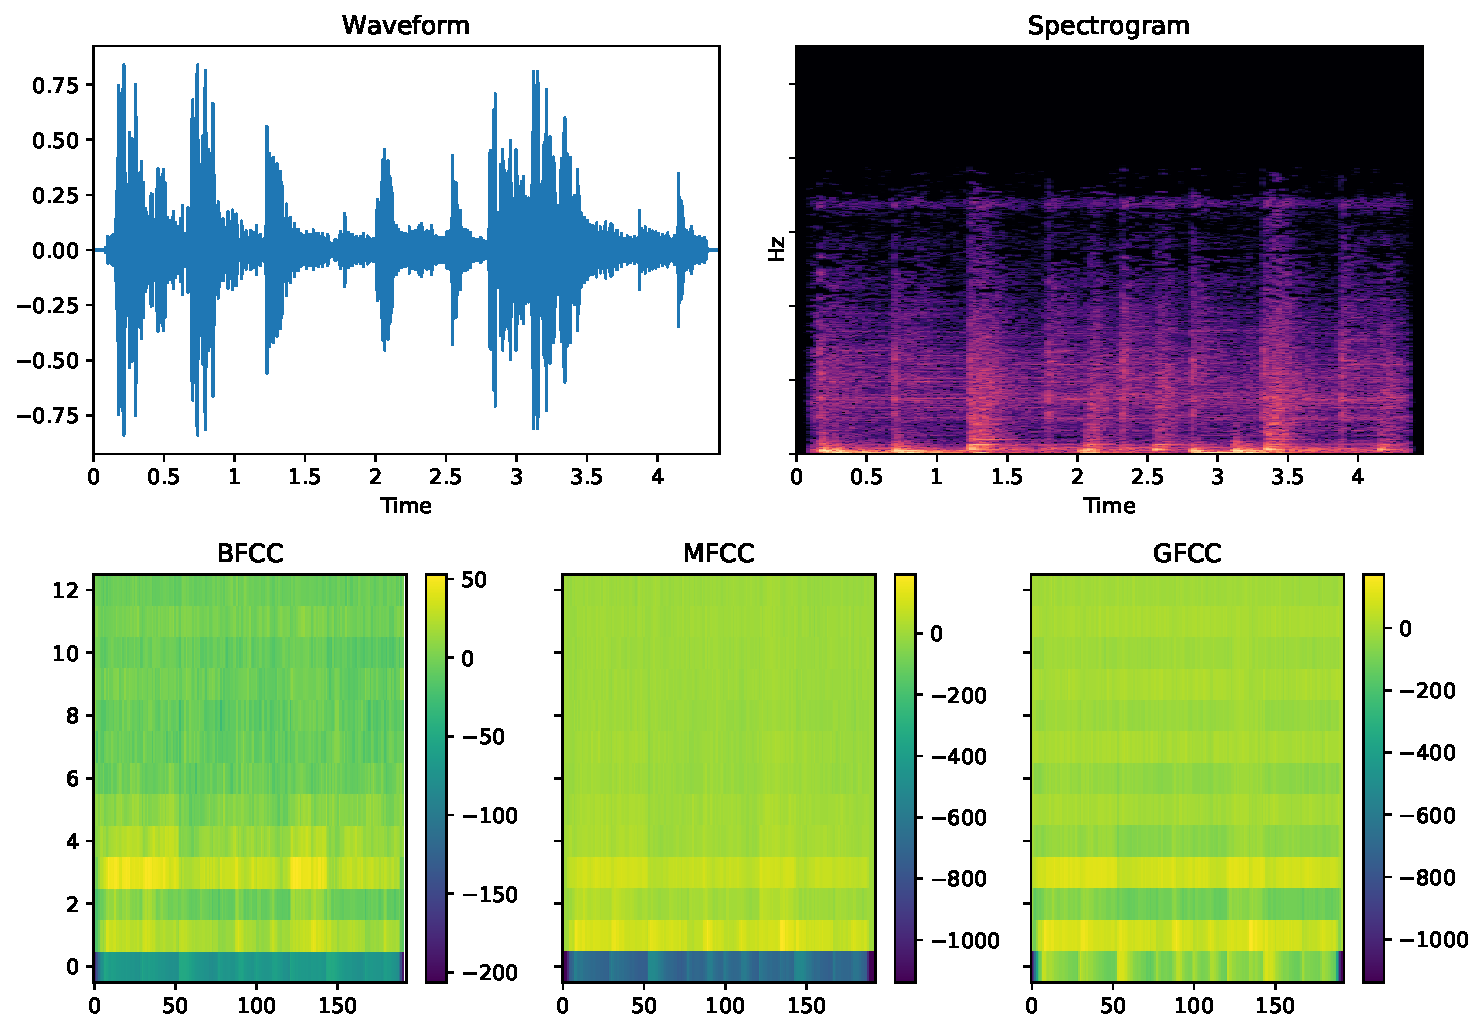
\includegraphics[scale=0.75]{ch05_pyconcat/figures/wave_spec_mfcc_bfcc.pdf}		
		\end{center}
		\caption[Waveform, Spectrogram, BFCC, MFCC and GFCC impressions of the ``Amen Break'' drum solo from ``Amen Brother'']{Waveform of drum break from ``Amen Brother'' (top-left). Power Spectrogram of waveform (top-right). BFCC coefficients 1-13 by frame number (bottom-left). MFCC coefficients 1-13 by frame number (bottom-centre). GFCC coefficients 1-13 by frame number (bottom-right)}
	\label{fig:bfcc_mfcc_gfcc_compared}
\end{sidewaysfigure}

%\begin{figure}
%	\begin{center}
%		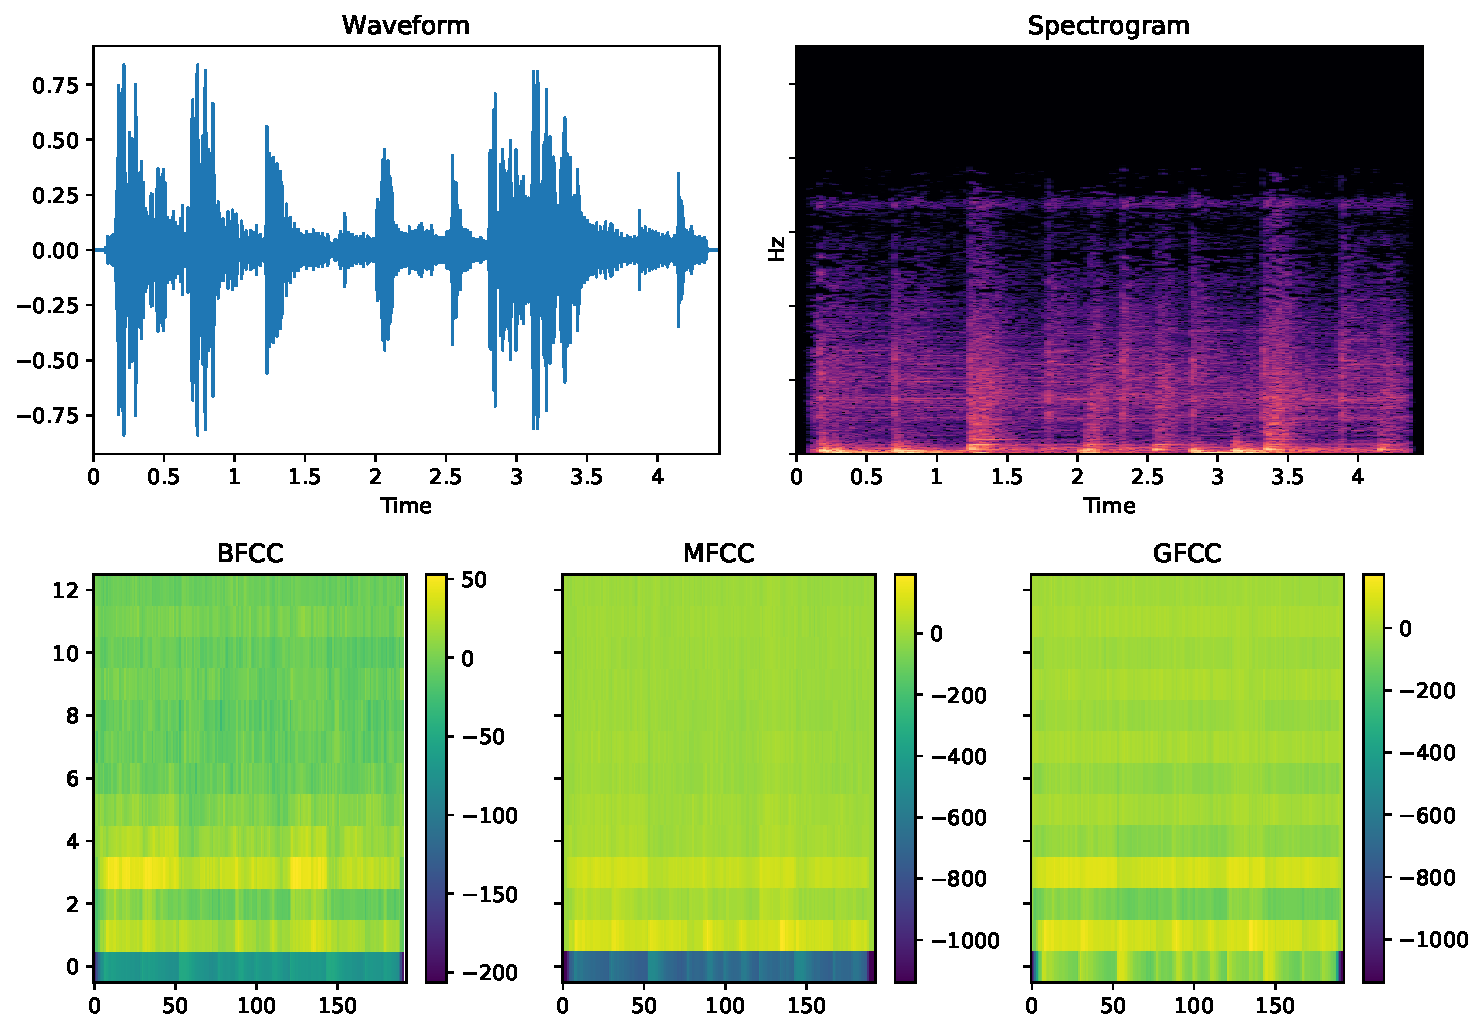
\includegraphics[width=1.0\textwidth]{ch05_pyconcat/figures/wave_spec_mfcc_bfcc.pdf}
%	\end{center}
%	\caption[Waveform, Spectrogram, MFCC and BFCC Representations]{Waveform of drum break from ``Amen Brother'' (top-left). Power Spectrogram of waveform (bottom-left). MFCC coefficients 1-13 by frame number (top-right). BFCC coefficients 1-13 by frame number (bottom-right).}
%	\label{fig:wave_spec_mfcc_bfcc}
%\end{figure}


Interpreting exactly the meaning of each of the MFCC coefficients (\figref{fig:bfcc_mfcc_gfcc_compared}) is not as simple as is examining each bin of an \acrshort{fft} for instance. However, in most discourse dealing with \acrshort{mfcc} analysis the emphasis appears to be on the first 13 coefficients as higher order coefficients are considered to contain increasingly redundant information. Additionally, the first coefficient is usually correlated most with the energy of the signal and is also frequently omitted in further usage.  We follow suit also, since we are already computing energy using the specially designed Stevens' Power Law descriptor.

{\renewcommand{\arraystretch}{1.5}
\begin{table} 
		\begin{tabular}{l l l l l}
\tabletop
Library & Language & MFCC & BFCC & GFCC\\
\tablemid
Aubio  \citep{Brossier2006} & C \& Pd & Yes  & No & No\\
MIR Toolbox \citep{Lartillot2008} & Matlab & Yes  & No & No\\
LibXtract \citep{Bullock2007} & Pd & Yes  & No & No\\
TimbreID \citep{Brent2010} & Pd & Yes  & Yes & No\\
Essentia \citep{Bogdanov2013} & C++ \& Python & Yes  & No & Yes\\
Librosa  \citep{Mcfee2015} & Python & Yes  & No & No\\
Madmom \citep{Bock2016} & Python  & Yes  & No & No\\
\tablebot
		\end{tabular}
		\caption[Availability of MFCC, BFCC and GFCC Descriptors in Common Audio Labelling Libraries]{Availability of \acrshort{mfcc}, \acrshort{bfcc} and \acrshort{gfcc} Descriptors in Common Audio Labelling Libraries.}
		\label{tab:library_summary}
	\par
\end{table}


\subsubsection{BFCCs}

If the \acrshort{mfcc} feature uses the Mel scale for warping the spectrum, then the extremely related \acrshort{bfcc} feature differs only in its warping procedure using the Bark scale. The Bark scale maps frequency to Barks using this formula:

\begin{equation}
\label{eq:High Frequency Content}	
b = [26.81*\frac{f}{(1960-f})]-0.53
\end{equation}

Aside from that the procedure is pretty much the same as for \acrshort{mfcc} computation. Overlapping filterbanks tuned to the the bark scale are applied to the spectrum, the logarithm is applied and finally the \acrshort{dct} transform is performed to produce the coefficients.

The \acrshort{bfcc} feature has not enjoyed the same level of popularity as its \acrshort{mfcc} counterpart, most probably since it is not available as an extractor in the major feature extraction and analysis environments (\tabref{tab:library_summary}).

The Mel scale is an extremely robust and reliable warping scale for many applications, but it is still prudent to experiment with other feature extractions methods depending on the application area its associated data. We decided to examine the applicability of the Bark scale following the findings of William Brent, who maintains that \acrshort{bfcc}s are the most accurate single feature in his own experiments in percussive timbre identification \citep{Brent2009, Brent2009a}. His TimbreID toolkit, due to its ease of use and implementation within the Pure Data environment has been popular in creative applications, and as a consequence his suggested usage of the \acrshort{bfcc} feature has been taken up in other works \citep{Monteiro2011, Neupert2013, Tomas2014}, including some tailored towards rhythm classification \citep{Miron2013, Vogiatzoglou2016, Jathal2017}, with the latter also reporting slightly better classification results over \acrshort{mfcc}s. Considering the frequent rhythmic purposes of our own research, and the percussive, attack quality of dance-oriented electronic music in general, it suggests applicability in our system.

{\renewcommand{\arraystretch}{1.5}
\begin{table} 
	\begin{centering}
	\small
	\texttt{%
		\begin{tabular}{l}
\tabletop
\tablemid
type = 'power' \\
weighting = 'linear' \\
lowFrequencyBound = 0 \\
highFrequencyBound = 8000 \\
numberBands = 26 \\
numberCoefficients = 13 \\
normalize = 'unit\_max' \\
dctType = 3 \\
logType = 'log' \\
liftering = 22 \\
\tablebot
		\end{tabular}
		}
		\caption[BFCC parameters for matching output of \cite{Ellis2005}]{BFCC parameters for matching output of \cite{Ellis2005}}
		\label{tab:bfcc_parameters}
	\par \end{centering}
\end{table}

While a consolidated \acrshort{bfcc} extractor doesn't exist in Essentia, a BarkBands filter does, and the algorithm structure in \figref{fig:mfcc_diagram} hints that all that is required is simply swapping the two filter types, which we did. What was a bit more difficult was verifying if the extractor was then outputting correct coefficients and comparable coefficients compared to other implementations - due to the lack of existing implementations. However, \cite{Ellis2005} has done some work on reproducing the feature of outputs of different implementations such as those found in \acrfull{htk} \citep{Young2002} or the Auditory Toolbox \citep{Slaney1998}, and has some routines for producing \acrshort{bfcc}s, so we decided to follow a similar procedure.

One of the first stumbling blocks came with the existing BarkBands filter, as it uses 27 pre-cooked Bark band frequencies that are hard-coded in the algorithm itself, rather than allowing parametric control of the lower and upper frequency bounds and the number of desired bands. To remedy this, we first created a TriangularBarkBands algorithm according to Ellis' specifications that provides precise parametric control of these crucial settings, in this way we can tweak settings to produce comparable feature outputs with Essentia. Next we modified a copy of the existing composite \acrshort{mfcc} algorithm and swapped in the TriangularBarkBands to create the new \acrshort{bfcc} extractor. After some experimentation we were able to achieve almost identical BFC coefficients as Ellis' ``Rastamat''\footnote{\url{http://www.ee.columbia.edu/ln/rosa/matlab/rastamat/}} implementation in Matlab (\figref{fig:matlab_bark}) using the parameter settings in \tabref{tab:bfcc_parameters}. With this implementation Essentia is now the only ``off the shelf'' feature extraction library that provides all three cepstrum descriptors.

\begin{figure}
	\begin{center}
		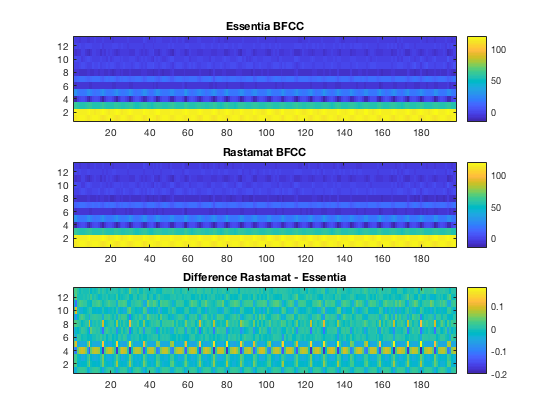
\includegraphics[width=1.0\textwidth]{ch05_pyconcat/figures/matlab_bark.png}
	\end{center}
	\caption[BFCC outputs with errors for Rastamat and our Essentia Implementations]{\acrshort{bfcc} outputs with errors for Rastamat and our Essentia Implementations}
	\label{fig:matlab_bark}
\end{figure}

\subsubsection{GFCCs}

Our final warped cepstrum feature is the \acrshort{gfcc} (or \acrshort{gtcc} to give its alternative acronym by some investigators \citep{Valero2012, Fathima2013}). The \acrshort{gfcc} derives its warping mechanism from the gammatone filter (\eqnref{eq:gammatone}), whose impulse response is purported to correlate closely with the auditory response of the cochlea in mammals \citep{Patterson1987, Valero2012}.

\begin{equation}
\label{eq:gammatone}	
g(t)=at^{n-1}e^{-2\pi bt}cos(2\pi ft + \phi)
\end{equation}

Here what we are seeing is basically a cosine waveform at a frequency $f$ with initial phase $\phi$ and amplitude $a$ modulated by the gamma function at order $n$ with a bandwidth $b$. Practically speaking, they are implemented using as set of \acrshort{erb} rectangular filters tuned to the gammatone properties. The computation is slightly more involved than the Mel or Bark approaches but in  Essentia, just like our port of the \acrshort{bfcc} algorithm, these filters are  modelled on a Matlab version made available in by \cite{Ellis2009}. who in turn formulated his solution as a response to the more computationally expensive routines available in Slaney's Auditory Toolbox \citep{Slaney1998}. 

 As \cite{Zhao2013} note, the \acrshort{erb} scale has finer resolution at lower frequencies (where pitch information is more compressed perceptually) than the Mel scale used in \acrshort{mfcc} computation. The other difference is the addition of a cubic root rectifier in place of the typical log. They posit that these adjustments over usual \acrshort{mfcc} approaches provide more robustness in the case of speaker identification in speech processing tasks. Indeed, \acrshort{gfcc} analysis has proved fruitful in many works dealing with speech \citep{Abdulla2002, Schl2007}, but has yet to prove widespread in musical or non-speech experiments. Recently however we have seen the introduction of \acrshort{gfcc} feature extraction in singer identification \citep{Cai2011}, structural segmentation \citep{Tian2016}, genre classification \citep{Johnson-Roberson2017, Grekow2017}, environmental sounds \citep{Valero2012} with improvements over classical Mel-based scaling approaches in many cases. 


\subsubsection{Tristimulus}

An interesting, alternative viewpoint of timbre, first proposed by \cite{Pollard1982}, takes inspiration from primary colour mixing model of light and attempts to model an equivalent for sound. Using information from the estimated fundamental frequency and harmonic peaks in the spectrum, the energy ratios of the first harmonic, the second, third and fourth harmonics and finally the rest of the harmonics form the three values of Tristimulus descriptor \citep{Peeters2004b}.

Tristimulus is obviously very useful for visualisation, as we can map it directly to colour \citep{Sequera2006}, or to 3-dimensional space  (\figref{fig:tristimulus}) without resorting to dimensional scaling. Also, in a more creative application of the feature, \cite{Fox2005a} use tilt data in an accelerator equipped glove for Tristimulus-based formant and timbre control of a synthesiser. 

Compared to more pitch ``agnostic'' timbral impressions such as cepstrum analysis, tristimulus features are more applicable for analysing signals with high degree of harmonicity, as \cite{Terasawa2006} note: 

\blockquote{\textit{
``[Tristimulus], however, is limited by the inability to represent inharmonicity and a rather arbitrary delineation of the three frequency components.''}
}

For succint and effective analysis of a broad range of signals Tristimulus should likely be aggregated with descriptors that are more suited for capturing those attributes, such as inharmonicity or spectral moments \citep{Peeters2004b,Chudy2010}.
 
\subsection{Musical Specific Descriptors}

\begin{figure}
	\begin{center}
		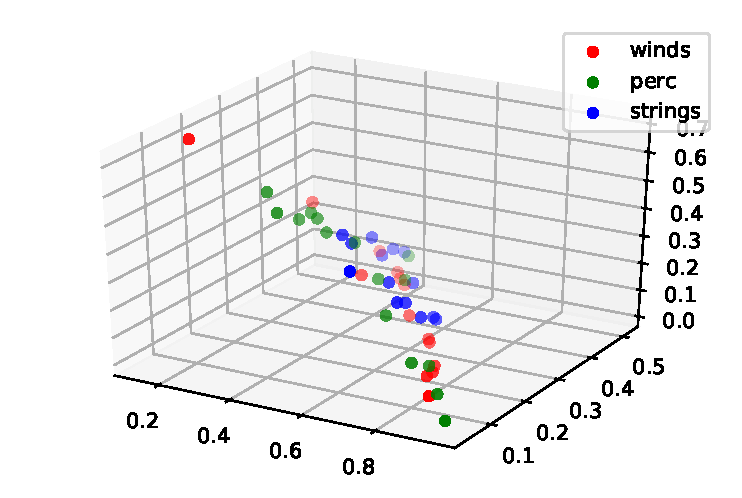
\includegraphics[width=0.75\textwidth]{ch05_pyconcat/figures/tristimulus.pdf}
	\end{center}
	\caption[Tristimulus plot for 3 different classes of instruments]{Tristimulus plot for 3 different classes of instruments, taken at random from the Philharmonica set}
	\label{fig:tristimulus}
\end{figure}

The features we have previously described and will evaluate in due course are extracted with the sole intention of matching target unit sounds with corpus units based on some perceived notion of ``timbre''. We distinguish here two features that are extracted with the intention of fulfilling more ``musical'' (of course timbre and music are inextricably intertwined) purposes such as:

\begin{enumerate}
  \item Pitch Tracking: Returning units that contain the same pitch, or transforming/post-processing units to contain the same pitch.
  \item Harmonic analysis: Returning units that containing similar harmonic profiles i.e. might contain similar tonality in terms of localised chord or overall key.
\end{enumerate}


\subsubsection{Fundamental Frequency and Pitch}

\acrfull{f0} detection or pitch tracking attempts to determine the lowest frequency within a signal, with the hopes that this matches the listeners perceptual impression of pitch \citep{Gerhard2003}. Algorithms for pitch detection exist in both the time and frequency domain. Time domain methods usually stem from some sort of autocorrelation of the signal, whereby the signal is compared with itself in increasingly delayed time lags to discover periodic repetitions whose reciprocal corresponds to the fundamental frequency given by $1/f = T$. Due to the harmonic nature of musical signals, autocorrelation methods often return octave errors, where multiples of the actual fundamental frequency are reported instead.

The well-known YIN\footnote{The name is derived from the yin and yang principle of contrary forces in Chinese philosophy, as the algorithm itself is a tradeoff between autocorrelation and cancellation.} algorithm \citep{DeCheveigne2002} addresses these errors and more by adding some correction stages such as absolute thresholding and parabolic interpolation, and is available within Essentia. \cite{Brossier2006} defines a YIN equivalent called PitchYinFFT in the frequency domain, taking advantage of convolution/multiplication equivalency to reduce some of the computation overhead inherent in the time domain method. Given the modular nature of feature extraction in Essentia and since we are already computing the spectogram for cepstrum analysis, it makes sense that we use this version for our pitch tracking needs.

\subsubsection{Chroma and (H)PCPs}

Just as the middle stage in the previous cepstrum analysis methods warped the frequency spectrum to a compressed non-linear scale, the chromagram feature also represents a collapse of the spectrogram (though without any further cepstrum transform), this time into musically relevant pitch classes based on \acrfull{pcp}s \citep{Fujishima1999} or \acrfull{hpcp}s \citep{Gomez2004} chroma extractors \citep{Orio2006}. The resulting feature contains the integrated intensities of the spectrum with respect to the 12 semitones of the diatonic scale assuming equal temperament, although further ratio resolutions (return vectors of size 24 or 48 for example) of the semitone are also used.

\acrshort{hpcp} computation, as proposed by \cite{Gomez2006} is carried out as follow. 

\begin{enumerate}
  \item Perform the \acrshort{stft}
  \item Locate peaks in the spectrum using a peak picking procedure as we saw in the onset detection stage (See \secref{sec:peak_picking}).
  \item Use the \acrshort{pcp} procedure to map the spectral peaks to folded intensities in a set containing the desired number of pitch classes.
  \item Normalise values based on the maximum.
\end{enumerate}

As the classification experiment will disclose, \acrshort{hpcp}s are less useful for timbral analysis, as it is not really their intended purpose. They are naturally effective features for systems that need to understand harmonic qualities such as chord recognition \citep{Fujishima1999} and key detection \citep{Gomez2004}. Indeed, within the GiantSteps project our colleagues have adapted customised key profiles that can extend to the stylistic peculiarities of tonality and key that pervade dance music \citep{Faraldo2016, Faraldo2017, Faraldo2017b}.

\subsection{Feature Combination and Evaluation}

To evaluate the ability of some of the features we have described here in classifying musically relevant timbres, we trained and tested two models with a number of classifiers. Our goal is not to provide a comprehensive work on timbral classification but rather serve as a broader sanity check to confirm two queries:

\begin{itemize}
  \item Are the features we have chosen appropriate for timbral classification and similarity analysis, and more specifically, analysis for rhythmic and percussive sounds?
  \item Do more exotic Cepstrum warping procedures like our implemented \acrshort{bfcc} and the \acrshort{gfcc} outperform the more commonplace \acrshort{mfcc}?
\end{itemize}

To address the requirements in our classification task two distinct datasets were compiled. The first set focusses on sections and instruments of the orchestra and the second focusses on percussive timbres of a typical drum set or drum machine.

\begin{figure}
	\begin{center}
		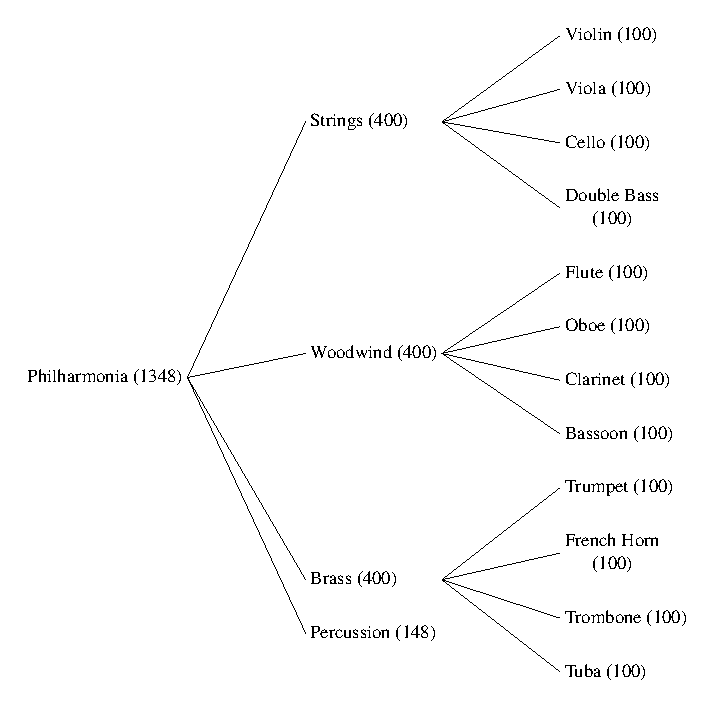
\includegraphics[width=0.8\textwidth]{ch05_pyconcat/figures/orch_distribution.pdf}
	\end{center}
	\caption[Summary Tree of Orchestral Samples for Classification]{Summary Tree of Orchestral Samples for Classification}
	\label{fig:orch_distribution}
\end{figure}

\paragraph{Orchestral Dataset}
\label{sec:orch_dataset}

The orchestral dataset comprises professionally recorded orchestral samples kindly made available for free download by London's Philharmonia Orchestra\footnote{\url{https://www.philharmonia.co.uk/explore/sound_samples}}, and has been used in a number of existing works for both analysis \citep{Hulshof2016, Donnelly2016, Pishdadian2017} and interactive performance \citep{Miller2010}. The total number of sound files exceeds well over 10,000 so we restricted ourselves to the standard instrumentation of the three choirs (strings, woodwinds and brass) as well as percussion, and omitted extended instruments such as guitar or banjo. All 148 percussion samples were selected from the set, and ranged from typical instruments such as the bass drum and cymbals to more exotic items like the washboard and whip. \figref{fig:orch_distribution} shows a tree structure summary of the distribution of the samples across instrumentation and the respective sections. 200 samples from each of the instruments were taken at random, with a wide variety of dynamics and articulations.

\paragraph{Drum Dataset}
\label{sec:drum_dataset}

The drum dataset was compiled to address better the rhythmic goals of this thesis and comprises over 1000 one shot samples of drum sounds. The samples themselves were sourced from freely availably libraries on the internet including one large repository provided by the popular musician focussed website Music Radar\footnote{\url{http://www.musicradar.com/news/drums/sampleradar-1000-free-drum-samples-229460}}. We have found one article in the literature \citep{Masood2015} that uses Music Radar samples for timbral classification of multiple instruments using a neural network. Our dataset contains a mixture of regular kit sounds and some percussion sounds from acoustic recordings as well as electronic drum machines like the Roland TR range. After verifying the trustworthiness with some random auditioning of the samples, we relied on the existing labelling in the filenames to divide up into appropriate classes for training and testing, which are summarised in the tree in \figref{fig:drum_tree}.


\subsubsection{Classifier Summary}

\begin{figure}
	\begin{center}
		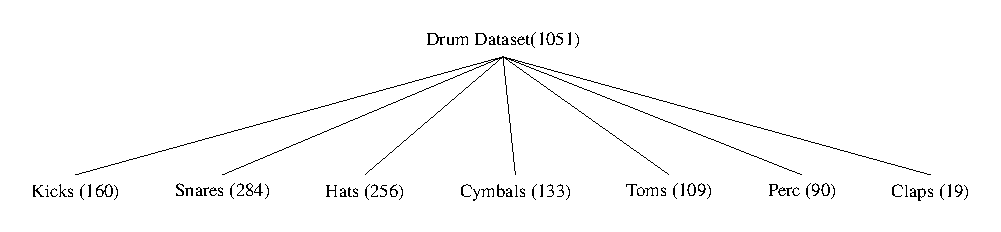
\includegraphics[width=1.0\textwidth]{ch05_pyconcat/figures/drum_distribution.pdf}
	\end{center}
	\caption[Summary Tree of Drum Samples for Classification]{Summary Tree of Drum Samples for Classification}
	\label{fig:drum_tree}
\end{figure}

For our classification and feature evaluation experiments we compared the performance of the various feature configurations on 3 distinct classifiers. We have relied on the availability of those available with "black-box" functionality in the scikit-learn \citep{Pedregosa2012} library for Python, and apart from some minor adjustment of high-level parameters we have not gone too deep into their inner workings.

\paragraph{Nearest Neighbours (\textit{k}NN)}

For any experiments involving supervised learning and classification of labelled observations, the \acrfull{knn} classifier should ideally be the first considered. \textit{k}NN invokes a voting based system where $k$ is the number of neighbouring instances that decide which class a new observation belongs to based on some distance metric. \textit{k}NN is attractive due to its conceptual simplicity, and has delivered favourable results in many timbre classification applications \citep{Herrera2002, Herrera2003, Herrera-Boyer2003, Mandel2005, Wang2006, Somerville2008}. Unfortunately it is a lazy form of learning, meaning all computation needs to be carried out when a new observation needs to be classified, thus it might not scale sufficiently depending on the problem application. In our evaluation we choose $k=1$ after  experimenting with $k=3,5$ and not achieving better accuracy.

\paragraph{Support Vector Machines} 

\acrfull{svm}s as a classification mechanism and in comparison to nearest neighbours methods are significantly more complex in their conception. In a nutshell, an SVM algorithm will try to find an idealised hyperplane that separates instances into multiclasses in multidimensional space \citep{Chang2008}. At lower dimensionality, linear separation is not always possible, so a ``kernel function'' is used to artificially transform the problem set to higher dimensionality for easier separation between the classes \citep{Xu2003}. Luckily the availability of libraries such as LibSVM \citep{Chang2011} (also integrated into scikit-learn) means this algorithm can be easily incorporated into classification experiments. SVM have been used successfully in classification of Western and Chinese classical instruments \citep{Liu2010a}, drum sounds \citep{Herrera2002, Herrera2003} as well as general instrument and timbre classification \citep{Herrera-Boyer2003, Krey2010, Agostini2003, Deng2008}.

\paragraph{Artificial Neural Networks}

\begin{figure}
	\begin{center}
		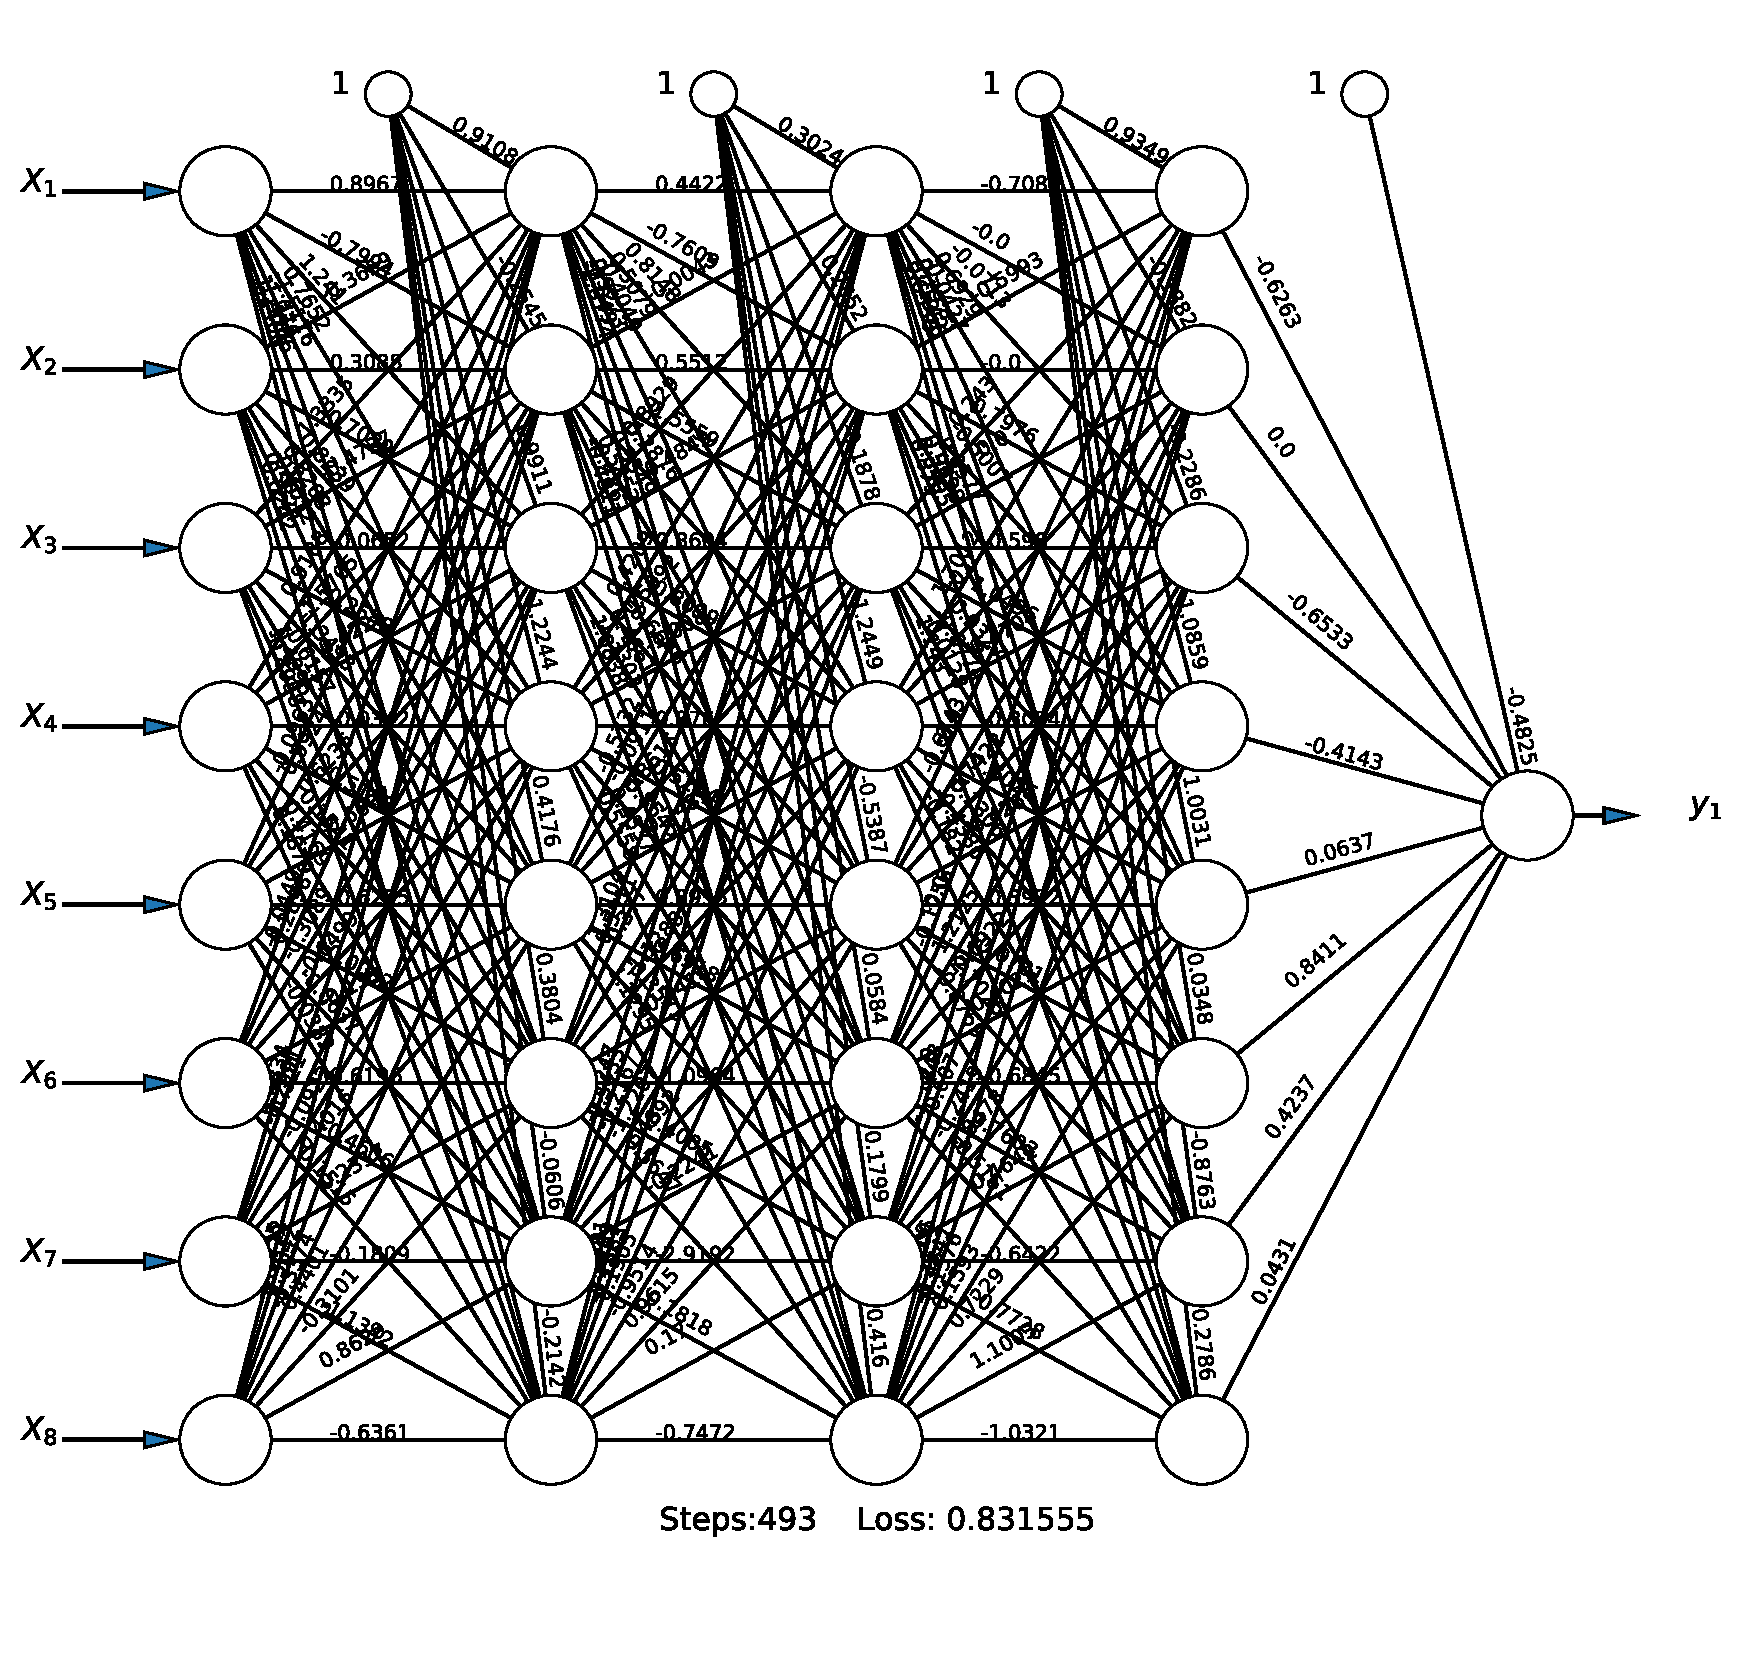
\includegraphics[width=0.8\textwidth]{ch05_pyconcat/figures/neural_network.pdf}
	\end{center}
	\caption[Input, Hidden and Output Layers for Multilayer Perceptron Classifier]{Input, Hidden and Output Layers for Multilayer Perceptron Classifier}
	\label{fig:neural_net}
\end{figure}

An \acrfull{ann} mimics the pattern recognition capabilities of the human brain, specifically through the use of the multilayer perceptron. Multiple layers of digital neurons - \acrshort{tlu}s that ``fire'' a value when a weighted sum of the inputs exceed a threshold value - are arranged in a fully-connected, feedforward (generally cycles aren't used) architecture \citep{Russell2002}. They can be trained to learn from example through the use of ``back-propagation'', a procedure that determines the error and distributes the blame back through the network so the weights can be adjusted to finally settle on minimal error \citep{Gurney1996}.

\figref{fig:neural_net} shows an example topology of a network trained with 3 hidden layers of 8 perceptron units for each of the 8 features chosen from the temporal and spectral feature classes (mean and variance for loudness, log-attack time, spectral centroid and flatness). Artificial neural networks are sensitive to feature scaling and disparate ranges, thus we standardised each feature for mean centred at $\mu=0$ and standard deviation at $\sigma=1$. 

\subsubsection{Results}

{\renewcommand{\arraystretch}{1.5}
\begin{table} 
	\begin{centering}
		\begin{tabular}{l l}
\tabletop
Feature Grouping & Features\\
\tablemid
Temporal (4) & loudness.mean (1), loudness.var (1)\\
		& logattacktime.mean (1), logattacktime.var (1)\\
Spectral (4) & flatness.mean (1), flatness.var (1)\\
		& logattacktime.mean (1), logattacktime.var (1)\\
\acrshort{bfcc} (26) & bfcc.mean (13), bfcc.var (13)\\
\acrshort{gfcc} (26) & gfcc.mean (13), gfcc.var (13)\\
\acrshort{hpcp} (24) & hpcp.mean (12), hpcp.var (12)\\
\acrshort{mfcc} (26) & mfcc.mean (13), mfcc.var (13)\\
\tablebot
		\end{tabular}
		\caption[Feature Configurations for Classifier Testing]{Feature Configurations for Classifier Testing}
		\label{tab:feature_groupings}
	\par \end{centering} 
\end{table}

To determine the interaction and ability of different feature sets  we divided the base level features into temporal, spectral, harmonic and timbral groupings and experimented with a number of combinations of these groupings (\tabref{tab:feature_groupings}).  In terms of preprocessing all features were normalised using min-max normalisation, except for the neural network which seemed to respond better to data standardisation versus normalisation. For each classifier 10-fold cross validation was performed, then the results were aggregated and reported along with their 95\% confidence interval.

\tabref{tab:orch_classification} shows the accuracy results for each classifier applied to the various configurations of descriptors when run on the orchestral dataset. The neural network and SVM returned the highest classification accuracy run on the whole collection of features using \acrshort{gfcc} cepstral analysis.

{\renewcommand{\arraystretch}{1.5}
\begin{table} 
	\begin{centering}
		\begin{tabular}{c c c c}
\tabletop
& \acrshort{knn} & SVM & ANN\\
\tablemid
Temporal               & 0.21 (+/- 0.03) & 0.24 (+/- 0.03) & 0.27 (+/- 0.05) \\
Spectral               & 0.50 (+/- 0.06) & 0.49 (+/- 0.04) & 0.55 (+/- 0.03) \\
Temporal+Spectral      & 0.62 (+/- 0.03) & 0.54 (+/- 0.06) & 0.67 (+/- 0.06) \\
\hdashline
BFCC                   & 0.89 (+/- 0.04) & 0.93 (+/- 0.04) & 0.93 (+/- 0.03) \\
BFCC+Temporal+Spectral & 0.91 (+/- 0.03) & 0.94 (+/- 0.03) & 0.95 (+/- 0.03) \\
\hdashline
GFCC                   & 0.91 (+/- 0.03) & 0.95 (+/- 0.02) & 0.95 (+/- 0.03) \\
GFCC+Temporal+Spectral & \textbf{0.92 (+/- 0.03)} & \textbf{0.96 (+/- 0.02)} & \textbf{0.96 (+/- 0.03)}\\
\hdashline
HPCP                   & 0.45 (+/- 0.04) & 0.44 (+/- 0.05) & 0.42 (+/- 0.05) \\
HPCP+Temporal+Spectral & 0.58 (+/- 0.04) & 0.69 (+/- 0.06) & 0.69 (+/- 0.05) \\
\hdashline
MFCC                   & 0.86 (+/- 0.03) & 0.90 (+/- 0.04) & 0.91 (+/- 0.04) \\
MFCC+Temporal+Spectral & 0.89 (+/- 0.02) & 0.93 (+/- 0.03) & 0.93 (+/- 0.03) \\
\tablebot
		\end{tabular}
		\caption[Mean Classification Accuracy and 95\% confidence interval for each classifier and feature configuration with the Orchestral Dataset]{Mean Classification Accuracy and 95\% confidence interval for each classifier and feature configuration with the Orchestral Dataset}
		\label{tab:orch_classification}
	\par \end{centering} 
\end{table}

\tabref{tab:drum_classification} shows the accuracy results for each classifier applied to the various configurations of descriptors when run on the drum dataset. \acrshort{knn} returned the highest classification accuracy once again with the whole collection of features using \acrshort{gfcc} cepstral analysis.

{\renewcommand{\arraystretch}{1.5}
\begin{table} 
	\begin{centering}
		\begin{tabular}{c c c c}
\tabletop
& \acrshort{knn} & SVM & ANN\\
\tablemid
Spectral               & 0.61 (+/- 0.08) & 0.56 (+/- 0.10) & 0.62 (+/- 0.12) \\
Temporal               & 0.37 (+/- 0.10) & 0.40 (+/- 0.08) & 0.44 (+/- 0.11) \\
Temporal+Spectral      & 0.66 (+/- 0.10) & 0.59 (+/- 0.09) & 0.69 (+/- 0.11) \\
\hdashline
BFCC                   & 0.86 (+/- 0.05) & 0.86 (+/- 0.07) & 0.83 (+/- 0.08) \\
BFCC+Temporal+Spectral & 0.85 (+/- 0.07) &\textbf{ 0.86 (+/- 0.06)} & \textbf{0.85 (+/- 0.09)} \\
\hdashline
GFCC                   & 0.86 (+/- 0.08) & 0.84 (+/- 0.08) & 0.84 (+/- 0.11) \\
GFCC+Temporal+Spectral & \textbf{0.87 (+/- 0.08)} & 0.86 (+/- 0.09) & 0.85 (+/- 0.12) \\
\hdashline
HPCP                   & 0.53 (+/- 0.17) & 0.55 (+/- 0.14) & 0.50 (+/- 0.14) \\
HPCP+Temporal+Spectral & 0.64 (+/- 0.12) & 0.71 (+/- 0.08) & 0.69 (+/- 0.08) \\
\hdashline
MFCC                   & 0.83 (+/- 0.10) & 0.84 (+/- 0.10) & 0.84 (+/- 0.09) \\
MFCC+Temporal+Spectral & 0.83 (+/- 0.09) & 0.85 (+/- 0.07) & 0.85 (+/- 0.04) \\
\tablebot
		\end{tabular}
		\caption[Mean Classification Accuracy and 95\% confidence interval for each classifier and feature configuration with the Drum Dataset]{Mean Classification Accuracy and 95\% confidence interval for each classifier and feature configuration with the Drum Dataset}
		\label{tab:drum_classification}
	\par \end{centering} 
\end{table}

The accuracy of classification is lower overall for our percussion dataset, which we can attribute as follows. Intuitively, the wider palette of sounds within an orchestra given the timbre of different instruments, dynamic ranges, articulations and so forth are bound to exhibit greater variance in the feature statistics that can aid us in separating the instances into their correct classes more easily. Looking at the confusion matrix (\figref{fig:drum_confusion}) for one of the test validations (GFCC+Temporal+Spectral trained with the \acrshort{svm}) we can see where the trends of the false positives lie. For example we some misclassification between toms and kicks which is to be expected - they are both lower frequency membranes without wires (unlike the snare). Also there is some misclassification of hi-hats and cymbals which are all broadband in their spectral profiles. It is also important to realise that, in drum machines at least, these sounds are generated using the same limit set of modules of oscillators and filters and so on, and I would challenge the most astute listener to blindly discriminate between many synthesised claps, snares, or hi-hats generated by  certain vintage drum machines.

\begin{figure}
	\begin{center}
		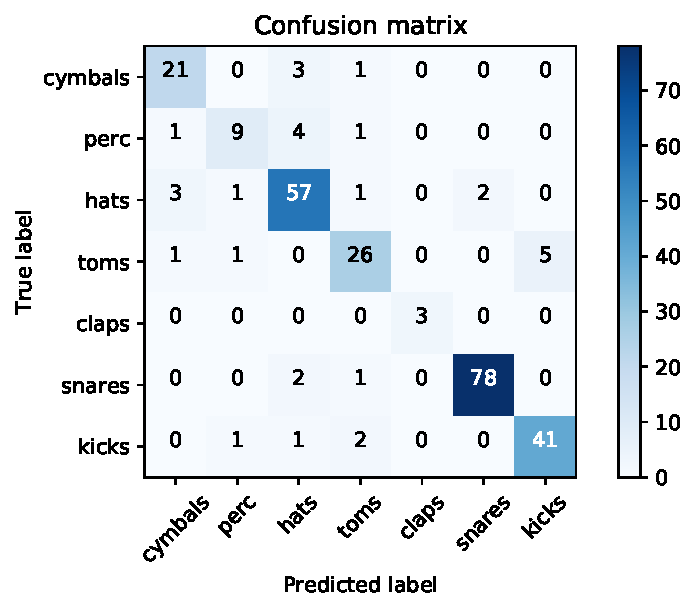
\includegraphics[width=0.8\textwidth]{ch05_pyconcat/figures/drum_confusion.pdf}
	\end{center}
	\caption[Confusion Matrix for Misclassification in Drum Dataset]{Confusion Matrix for Misclassification in Drum Dataset}
	\label{fig:drum_confusion}
\end{figure}

From these two experiments we can draw some conclusions. Firstly, cepstral methods alone are extremely robust descriptors on their own, with temporal and spectral additions to the configurations only contributing a few percent improvement to the overall accuracy scores in all cases. However, combining the full set of features does return the highest classification accuracy for both datasets. The second conclusion that we can draw is that alternative approaches to cepstral analysis using the Bark scale and Gammatone/ERB filterbanks do improve over classical Mel approaches.  Finally of these two cepstral methods, the \acrshort{gfcc} based has slight advantage over \acrshort{bfcc}, and probably for good reason - its gammatone filter was first proposed as an improvement to existing Critical Band scaling methods and supposedly more grounded in models of the auditory filter system. In turn, the Bark scale itself was proposed to address certain limitations with the Mel scale, and our results reflect this progression. We would stress that these methods be given serious consideration in any classification experiment for comparison and raising their reputation amongst wider research.

\section{Combining Sounds Algorithmically - Unit Selection}

Unit selection solves the the problem of determining what sounds to select from the corpus and the systematic structuring of the selected sounds for outputting logical concatenated sequences, or as Schwarz defines:

\blockcquote[]{Schwarz2006b}{``\textit{[Concatenative sound synthesis uses] a unit selection algorithm that finds the sequence of units that match best the sound or phrase to be synthesized, called the target. The selection is performed according to the descriptors of the units, which are characteristics extracted from the source sounds, or higher level descriptors attributed to them.}''} 

 Many unit selection schemata have been proposed and there exists no standard or best method. However some specific procedures have presented themselves repeatedly which we will summarise here:

\subsection{Linear Search}

At the most basic level a linear search criteria for unit selection simply computes the (dis)similarity of every unit in the target sequence with every possible unit in the corpus, according to some distance measure \citep{Schwarz2011}. For example, a weighted variation of Euclidean could be applied (taking care to normalise the feature vectors) that would allow the composer to place emphasis on certain features in the similarity computation as given by \eqnref{eq:linear_search}.

\begin{equation}
\label{eq:linear_search}
d(t^i, c^j) = \sqrt{\sum_{k=0}^{K-1}w_k(t^i_k-c^j_k)^2}
\end{equation}

Here $d(t^i, c^j)$ refers to the distance or dissimilarity between a target unit $t^i$ and a corpus unit $c^j$, index $k$ represents the individual feature value from the full set of $K$ features and $w_k$ represents a weighting to be applied to that feature during the distance computation. The closest corpus unit $s$ that should be selected for concatenation is then given by \eqnref{eq:linear_search_argmin}.

\begin{equation}
\label{eq:linear_search_argmin}
s = \operatorname*{arg\ min}_{0<j<N}\ d(t^i, c^j)
\end{equation}

 It is a conceptually simple and robust technique that has been applied in numerous systems (or at least non-weighted Euclidean) \citep{Dannenberg2006, Maestre2006, Sturm2006, Collins2007,  Stoll2013}. In fact, for ease of implementation, we have applied the linear search method ourselves in developing a real-time system for concatenative synthesis of rhythms as described in \citep{Nuanain2016a, ONuanain2017a}, which we examine in more depth in \chapref{chap:rhythmcat}. The overlying problem with this approach is that it only considers the disparity between the target and the corpus unit, and neglects treating the continuity or context of consecutive units within the output sequence. Depending on the size of the corpus it may also be prohibitively slow (but not in our informal usage, at least not compared to \acrshort{hmm}s), which can be remedied by applying a structure such as a \textit{k}-d Tree.

\subsubsection{Faster Search with \textit{k}-D Trees}

As \cite{Collins2007} and \cite{Dannenberg2006} have noted, the brute force nature of exhaustive linear search computation may not lend itself to scalability for larger datasets. The former suggests using \textit{k}-D Tree structures for more strategically optimising the search process, and has also been utilised in systems by \cite{Schwarz2009}, \cite{Einbond2010}, \cite{Stoll2013} and \cite{Klugel2014}.

A \textit{k}-D Tree organises points in space with a binary tree by successivly cycling through each dimension of the problem space (its full name is \textit{k}-Dimensional Tree), splitting the data at its median and assigning the two newly partitioned sets to the branches of the nodes at each level. The branching aspect of binary search trees allows us to eliminate vast portions of the search space when performing nearest neighbour searches. 

\begin{figure}
	\begin{center}
		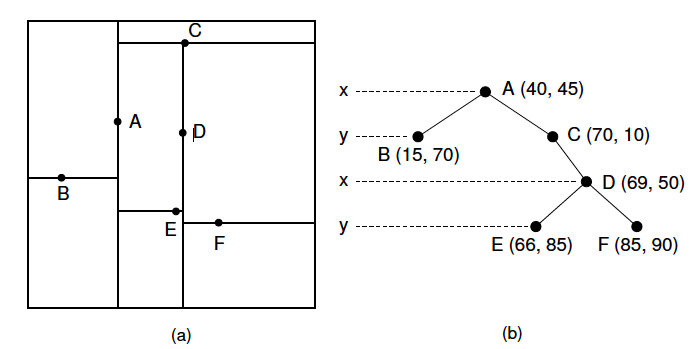
\includegraphics[width=1.0\textwidth]{ch05_pyconcat/figures/kdTree.png}
	\end{center}
	\caption[]{Hyperplane division (left) and binary tree (right) arrangement of 2-dimensional dataset with a \textit{k}-D Tree of depth 4. The origin is the top left and the size of the grid is 128x128 units. Image from Indiana University.}
	\label{fig:markov_unit}
\end{figure}

It is important to realise that they are only approximate solutions so they may not return the actual nearest neighbour (which is in an important factor to consider if it is to be used for accurate classification). A new instance may be routed down a branch too hastily based on its proximity in a single dimension even though the closest match based on the combined Euclidean distance may  belong to a different branch. Also, as \cite{Russell2002} stress, \textit{k}-D Trees are only useful so long as the number of examples exceeds the number of dimensions in the problem space, otherwise it is no more efficient than exhaustive, linear scanning. Many \textit{k}-D Tree inspired \acrfull{ann2} algorithms exist for dealing with high dimensionality problem domains, at a possible sacrifice in accuracy (it may not return the exact nearest neighbour). For instance in OpenCV a fast approximate \textit{k}-D Tree is implemented using a Best-Bin-First algorithm \citep{kaehler2016learning}. In PyConcat we avail of the implementation in the SciPy scientific package for python \citep{Scipy2014}.

\subsection{Unit Selection with Viterbi Decoding of Hidden Markov Models}
\label{viterbi_unit_selection}

The Viterbi algorithm was first applied by Hunt for the purposes of speech synthesis by performing unit selection of speech phonemes samples from a prior corpus \citep{Hunt1996}. It was then adopted for musical purposes by Diemo Schwarz in his Caterpillar System \citep{Schwarz2003}. By representing a unit selection system as a Hidden Markov Model we can not only consider the disparity between the target and corpus unit (encoded in the emission matrix) but also the “best fit” of continuity between two consecutive units in the output sequence as determined by the transition matrix of the hidden states (\figref{fig:markov_unit}).

As with shortest path problems, unit selection requires finding the \textit{minimisation} of a set of \textit{costs} \citep{Hunt1996}, namely the target cost $C^{t}$ between target and corpus units (\eqnref{eq:target_cost}, which is an identical derivation to \eqnref{eq:linear_search} in the linear search method) and the concatenation cost $C^{c}$ (\eqnref{eq:concatenation_cost}) between the consecutive concatenated units \citep{Schwarz2003}. This is in contrast to usual goal of Markov processes which of course is concerned with \textit{maximisation} of probabilities. 

A linear combination is finally performed with weights $w^{t}$ and $w^{c}$ to give the total cost $C$ (\eqnref{eq:total_cost}) . The constituent costs themselves are derived by computing the dissimilarity between the feature vectors of the associated units using a suitable distance metric and a set of $w_k$. The feature sets and accompanying weights can (and typically do) differ for the two different cost functions. 

\begin{equation}
\label{eq:target_cost}
C^{t}(t^i, c^j) = \sqrt{\sum_{k=0}^{K-1}w_k(t^i_k-c^j_k)^2}
\end{equation}

\begin{equation}
\label{eq:concatenation_cost}
C^{c}(c^j, c^j-1) = \sqrt{\sum_{k=0}^{K-1}w_k(c^j_k-c^{j-1}_k)^2}
\end{equation}

\begin{equation}
\label{eq:total_cost}
C = w^t.C^t + w^c.C^c
\end{equation}

One of the motivations for working with more complex unit selection schemes like \acrshort{hmm}s is that we can specify what we consider important for target cost computation separately to the concatenation cost computation by weighting accordingly or even choosing completely different features sets. For example, in speech synthesis we might choose features and weightings for the target cost that prioritises matching of length and linguistic context versus more prosodic configurations for the concatenation cost that encourage stability of energy and pitch.

\subsection{Constraint Satisfaction}

Schwarz notes, however, that the \acrshort{hmm} approach can be quite rigid for musical purposes because it produces one single optimised sequence without the ability to manipulate the individual units. To address these limitations, he reformulates the task into a constraint-satisfaction problem, which offers more flexibility for interaction. A constraint-satisfaction problem models a problem as a set of variables, values, and a set of constraints that allows us to identify which combinations of variables and values are violations of those constraints, thus allowing us to quickly reduce large portions of the search space \citep{Nierhaus2009}. 

\cite{Zils2001} first introduced constraint satisfaction for concatenative synthesis in what they describe as musical mosaicking - or, to use their portmanteau - musaicing. They define two categories of constraints: segment and sequence constraints. Segment constraints control aspects of individual units (much like the target cost in an \acrshort{hmm}-like system) based on their descriptor values. Sequence constraints apply globally and affect aspects of time, continuity, and overall distributions of units. The constraints can be applied manually by the user or learned by modelling a target. The musically tailored “adaptive search” algorithm performs a heuristic search to minimise the total global cost generated by the constraint problem. One immediate advantage of this approach over the \acrshort{hmm} is the ability to run the algorithm several times to generate alternative sequences, whereas the Viterbi process always outputs the most optimal solution. 

\section{Extensions to Hidden Markov Model-Based Unit Selection}

The singular output issue that Schwarz raised as a result of \acrshort{hmm}-based unit selection piqued our interest as we were delving into the specifics of unit selection  of concatenative synthesis ourselves. While it seems like an ideal mechanism for capturing the deep connectionist and interdependent arrangement of units that a successful and natural synthesis should ideally exhibit, it also runs counter productive to the very musical goals of creating and exploring heterogenous variations of a motif or loop.

To solve this limitation we propose a new method of \acrshort{hmm}-based unit selection that can return the \textit{k}-Best concatenated sequences given a target, a corpus of sounds and the number of desired sequences $k$ \citep{Nuanain2017}. Before this can be introduced however, we need to examine \acrshort{hmm}s and the Viterbi algorithm in more depth, which until now hasn't been treated with sufficient rigour. 

\subsection{Hidden Markov Models}

Recall from \chapref{chap:symbolic} that a Markov chain is a probabilistic system that satisfies the Markov property of memorylessness. It consists of a set of discrete states with each state having an associated probability weighting of moving to every other state in the system. At any point in discrete time, the probability of a future event is solely determined by the current state of the system without knowledge of past events (see \eqnref{eq:markov}).

A hidden markov model $\lambda = (A, B, \pi)$ extends the concept of a Markov chain by considering the transition states as hidden \citep{Rabiner1989}. The hidden states have a  transition matrix $A$ as before, but each hidden state also emits an observable symbol from a set of symbols that have a probability distribution encapsulated in an emission matrix $B$. Finally, to initiate the \acrshort{hmm} there also exists the initial probability distribution $\pi$, which determines the probability of which state to commence. 

The subtleties of Hidden Markov Models don’t become immediately clear until we start working with some common problems and especially their role in sound and music analysis and generation, but there are three traditional problems that are usually studied, as identified by Rabiner in his tutorial \citeyearpar{Rabiner1989}.

\begin{enumerate}
  \item \textit{Evaluation}  - Given an observable sequence of emissions $O = (O_1, 0_2, O3,..., O_T)$, what is the probability that the sequence was generated by a certain model $\lambda$. This is particularly useful when benchmarking or comparing different models. 

\item \textit{Decoding} - Given an observable sequence of emissions $O = (O_1, 0_2, O3,..., O_T)$, what is the most like sequence of hidden states that produced that observation $O$.

\item \textit{Learning or Training} - Given a model with its parameters $\lambda = (A, B, \pi)$ and an observable sequence of emissions $O = (O_1, 0_2, O3,..., O_T)$, how do we adjust the parameters to maximise the probability of the observable sequence $O$.
\end{enumerate}

\subsection{The Viterbi Algorithm}

The Viterbi algorithm solves the decoding problem in \acrshort{hmm}s \citep{Rabiner1989}, namely, for a given observation sequence $O = (O_1, 0_2, O3,..., O_T)$  we wish to determine the highest probable hidden state sequence $S = (S_1, S_2, S3,..., S_T)$ that would produce output $O$ given by:

\begin{equation}
\label{eq:Precision}	
S*=argmax (P(S|O))
\end{equation}  

A brute force solution applied to a $T$ observations over $N$ states would involve computing all the cartesian products of the possibilities; $N^T$ involving exponential time complexity. Viterbi’s algorithm enables us to reduce this complexity to $O(T.N^2)$, using dynamic programming techniques. Rather than exhaustively computing all the possibilities, we maintain two data structures alpha ($\alpha$) and phi($\phi$). At any point $t$ in the sequence to be decoded, we store the score of the maximum probability for emitting the observed symbol for each hidden state, along with the index or argument of the maximum probable state that led there. To get the optimal state sequence we get the index of the final highest scoring hidden state and backtrack through the $phi$ structure beginning with that index, returning the accumulated list. We can express this formally in the recurrence expression \ref{eq:markovstart}-\ref{eq:markovend}.

In the initialisation of the algorithm we use the initial probabilities and the observed symbol to calculate the starting probabilities of each hidden state in $\alpha$, and, as there can be no previous states, $\phi$ is set to 0.

The recursion step continues until $T$, the length of the observed sequence. We first calculate the maximum of the probability of each previous state multiplied by the transition probability to the current state. The winning maximum probability is multiplied by the emission probability of the observed symbol and stored in $\alpha$ while the index of that winning previous state is logged in $\phi$. 

The elegance of the Viterbi algorithm should be apparent here. Rather than computing the $N^{t-1}$ possible combinations of all the previous states, dynamic programming is used to store the result of the calculations in a matrix for later retrieval. 

When recursion halts, the highest final probability is computed and its index is used finally the backtrack through the state machine and thus returning $S^*$, the sequence of highest scoring hidden states that most likely produced the observed sequence $O$.

\newlist{inlinelist}{enumerate}{1}
\setlist[inlinelist,1]{%
  label=\arabic*),
}

\setlength{\parindent}{1cm}

\indent
%\small
{
\begin{align}
\intertext{ \indent \textbf{1) Initialisation:} $t=1$}
			\alpha_1(i) &= \pi_{i}B_{i}(O_1)\qquad1<i<N \nonumber \\
			\phi_1(i) &= 0 \label{eq:markovstart} \\
\intertext{ \indent \textbf{2) Recursion:} $t=2,...,t=T$}
			\alpha_t(j) &= max_{i\in N}(\alpha_{t-1}(i)A_{ij}B_{j}(O_{t}))\qquad1<j<N \nonumber \\
			\phi_t(j) &= argmax_{i\in N}(\alpha_{t-1}(i)A_{ij})\qquad1<j<N\\
\intertext{ \indent \textbf{3) Termination:}}
			p^* &= max_{i \in N}(\alpha_T(i)) \nonumber \\
			S^*_{T} &= argmax_{i \in N}(\alpha_T(i))\\
\intertext{ \indent \textbf{4) Backtracking:} $t=T-1,...,t=1$}
			S^*_{T} &= \phi_t+1(S^*_{t+1}) \label{eq:markovend}
\end{align}
}

\normalsize

The Viterbi algorithm has been around for quite a while now, and implementations exist in many frameworks and programming languages \citep{Bird2016, Gueguen2005}. It is a fundamental technique in bioinformatics and natural language and speech processing. \acrshort{pos} tagging for example, uses a \acrshort{hmm} trained on a large corpus of text with each word labelled with its constituent part of speech (e.g. noun, verb, article etc.). It proves more robust results in identifying new samples of text, as the transition matrix helps determine the context of each word within the sequence. 

We have provided a reference implementation of the single output probabilistic Viterbi as part of our ongoing \textit{k}-Best Viterbi work\footnote{\url{https://github.com/carthach/kBestViterbi/blob/master/kBestViterbi.py}}. An important caveat in the implementation of \acrshort{hmm} software is the possibility of numerical underflow due to multiplication of ever decreasing minute probabilities, for this reason programmers typically convert to log-space for allowing addition instead, which we also allow the option of.

{\renewcommand{\arraystretch}{1.5}
\begin{table} 
	\begin{centering}
	\footnotesize
	\texttt{%
		\begin{tabular}{l}
\tabletop
\tablemid
$O$ = (`normal', `cold', `dizzy')\\
$S$ = (`Healthy', `Fever')\\
$\pi$ = \{`Healthy': 0.5, `Fever': 0.4\} \\
$A$ = \{ \\
`Healthy' : \{`Healthy': 0.5, `Fever': 0.4\} \\
`Fever' : \{`Healthy': 0.4, `Fever': 0.6\} \\
 \} \\
$B$ = \{ \\
`Healthy' : \{`normal': 0.5, `cold': 0.4, `dizzy': 0.1\} \\
`Fever' : \{`normal': 0.1, `cold': 0.3, `dizzy': 0.6\} \\
 \} \\ 
\tablebot
		\end{tabular}
		}
		\caption[BFCC parameters for matching output of \cite{Ellis2005}]{\acrshort{hmm} parameters for Wikipedia Viterbi decoding example}
		\label{tab:hmm_parameters}
	\par \end{centering}
\end{table}

\figref{fig:viterbi_basic} shows a trellis diagram showing the highlighted trace of the decoded path ($S = (0, 0, 1)$), for the observed sequence $O = (0, 1, 2)$ (or `normal', `cold' and `dizzy' to give it its string labels) along with its calculations, computed by the Viterbi algorithm through the state space of the example problem in the Wikipedia article on Viterbi decoding \footnote{\url{https://en.wikipedia.org/wiki/Viterbi_algorithm}}. The parameters of the model are given in \tabref{tab:hmm_parameters}. Notice how the dynamic programming stage intuitively computes and stores the necessary probabilities for each state at each time step through the trellis.

\begin{figure}
	\begin{center}
		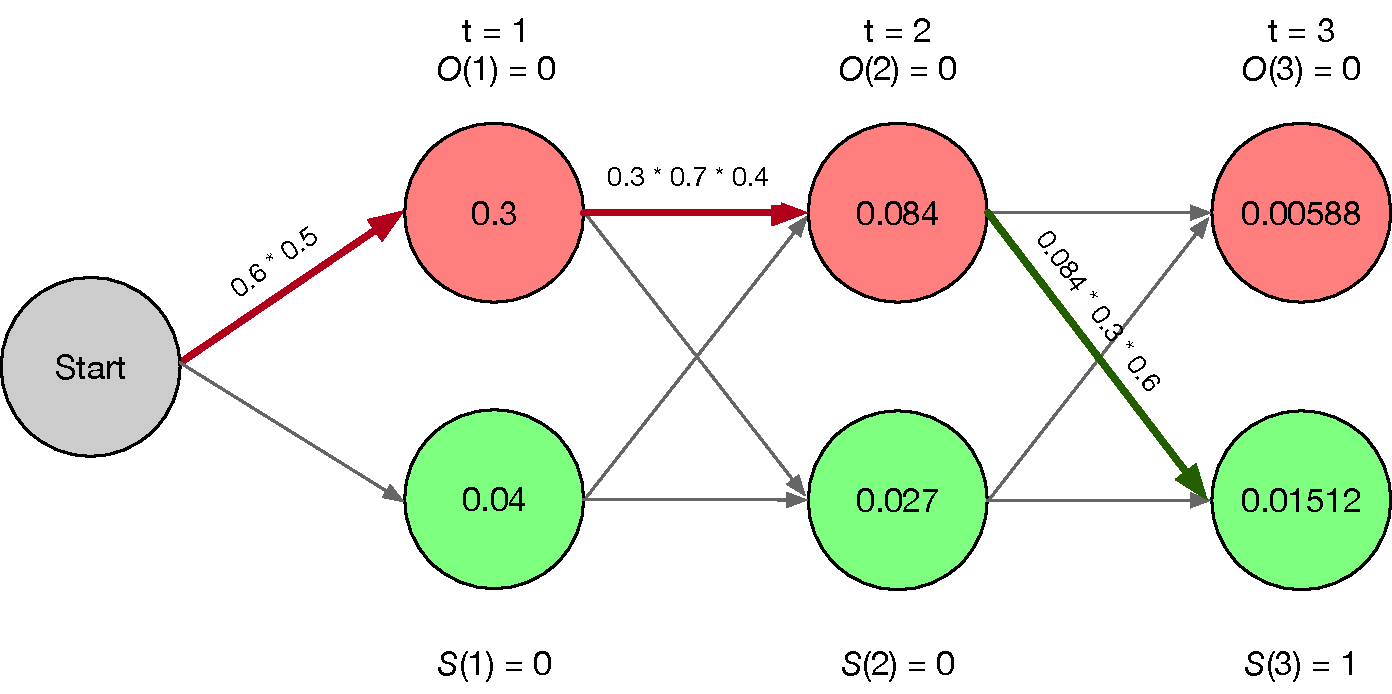
\includegraphics[width=0.85\textwidth]{ch05_pyconcat/figures/regular_viterbi.pdf}
	\end{center}
	\caption[Viterbi decoding of Wikipedia example using our decoder]{Viterbi decoding of Wikipedia example using our decoder}
	\label{fig:viterbi_basic}
\end{figure}

\subsection{HMMs in Musical Applications}

\acrshort{hmm}s' facility for pattern recognition has been exploited for computational musical tasks. Score following, for instance, tries to consolidate the position of a live performance of a musical piece with its score representation automatically \citep{Orio2003}. Using Viterbi decoding, an alignment can be established by extracting features for the observed live performance, and comparing them against idealised features within the model to return the expected location of the performance within the score.

\acrshort{hmm}s also lend themselves quite naturally to the task of chord recognition \citep{Papadopoulos2007, Cho2010, Sheh2003}. The former demonstrate a method whereby they compare the \acrshort{pcp} representation of the signal corresponding to 24 possible chord labels (12 notes for major and minor) indicated by the emission matrix, coupled with the most probable chord sequence defined in the transition matrix, derived from prior musical knowledge or training on musical scores and transcriptions.

Compared to Markov chains, \acrshort{hmm}s have been exploited somewhat less in generative or compositional applications (apart from concatenative synthesis, which we will describe presently). Some methods however are summarised in \citep{Fernandez2013} and \citep{Nierhaus2009}, with the latter making the observation that “when applied to algorithmic composition, \acrshort{hmm}s are appropriate to add elements to an existing composition”. 

\subsection{Adjusting Viterbi to Handle Unit Selection in Concatenative Synthesis}

As already stated, Markov systems try to maximise probabilities while concatenative synthesis systems try to minimise cost. The costs should be pre-computed by calculating the target cost $C^{t}$ for every target unit $t_i$ and database unit $c_j$, and the concatenation cost $C^{c}$ for every combination of unit $c_j$. These costs form the emission matrix $A$ and transition matrix $B$ parameters for our \acrshort{hmm} respectively. We can then discard the initial probability matrix $\pi$ and reformulate the Viterbi algorithm with the necessary changes for cost minimisation as in expression \ref{eq:concat_start}-\ref{eq:concat_end}. Note that the recursion and termination steps now use the $min$ and $argmin$ function and sum the final costs. 

\setlength{\parindent}{1cm}

\indent
%\small
{
\begin{align}
\intertext{ \indent \textbf{1) Initialisation:} $t=1$}
			\alpha_1(i) &= B_{i}(O_1)\qquad1<i<N \nonumber \\
			\phi_1(i) &= 0 \label{eq:concat_start} \\
\intertext{ \indent \textbf{2) Recursion:} $t=2,...,t=T$}
			\alpha_t(j) &= min_{i\in N}(\alpha_{t-1}(i)+A_{ij}+B_{j}(O_{t}))\qquad1<j<N \nonumber \\
			\phi_t(j) &= argmin_{i\in N}(\alpha_{t-1}(i)+A_{ij})\qquad1<j<N\\
\intertext{ \indent \textbf{3) Termination:}}
			p^* &= min_{i \in N}(\alpha_T(i)) \nonumber \\
			S^*_{T} &= argmin_{i \in N}(\alpha_T(i))\\
\intertext{ \indent \textbf{4) Backtracking:} $t=T-1,...,t=1$}
			S^*_{T} &= \phi_t+1(S^*_{t+1}) \label{eq:concat_end}
\end{align}
}

\normalsize

\subsection{Exploring Alternatives in HMMs}

One of the most thorough and cited articles dealing with \textit{k}-Best or, ``List Decoding'' as the author describes it, has been provided by \citep{Seshadri1994} who proposes two different methods to extend the regular Viterbi algorithm to multiple output. These methods he clarrifies  as operating in parallel or serial.  We summarise these methods here, and provide an implementation of the parallel approach for unit selection and concatenative synthesis.

As we were implementing the Parallel Decoder, we begin to notice the comparisons between the search process Viterbi takes through the hidden state space in a \acrshort{hmm} and the way that shortest path algorithms such as Dijkstra's find the path of least resistance through an acyclic directed graph, as we already saw in the computation of the direct-swap distance in \chapref{chap:symbolic}. In fact there are methods in graph research that can retrieve the k-Shortest Paths sequentially. To this end, we also demonstrate a method of reformulating a cost-based \acrshort{hmm} used in concatenative synthesis as a directed acyclic graph in order to avail of shortest path methods.

\subsubsection{Parallel Decoder}

The Parallel decoder \citep{Seshadri1994} or \acrfull{lva} is so-called because, instead of keeping track of the winning path leading into each state at time step $t$, it now stores the top $k$ paths leading into the states in one pass through the state space or trellis. This is distinct from the serial decoder which takes several passes through the trellis in order to return multiple candidates.

To convert the regular Viterbi decoder to a \textit{k}-Best Parallel decoder. the following steps are required.

\begin{enumerate}
  \item Expand the $\alpha$ and $\phi$ matrices of the \acrshort{hmm} to account for $T*N*K$ entries that correspond to $T$ discrete steps, $N$ states and $K$ sequences.
  \item When computing the probabilities of the transitions from the previous states leading into the current state as per the recursion step in the equation, insert them into a continuously sorting data structure like a priority queue\footnote{ A heap queue is a binary tree with the special condition that every parent has a value less than or equal to that of its children (this is a minimum queue, a maximum is naturally the inverse). The important function in our case is the push function, which adds items to the tree and maintains the sorted heap property in $O(log n)$ time. } (we use Python's \textit{heapq})
  \item Remember that there is now the possibility of a previous state leading to the current state more than once (because that previous state now also has $k$ previous states that are potentially high probability). Thus we need to another structure (such as a dictionary) to keep track of the ranking of multiple probabilities of the same previous state if it enters the current state more than once.
  \item At the termination step insert the final probabilities into the queue to find the final top \textit{k} scoring paths.
  \item Backtrack as before while taking care to adhere to the ranking of multiple instances of the same previous state.
\end{enumerate}

Curiously, we couldn't find fully-formed implementations exist for the Parallel decoder, at least not in any usable state of reproducibility, so once again we have implemented and made available ourselves a version in Python. \figref{fig:viterbi_parallel} shows how our newly implemented Parallel decoder computes the first and second highest probability paths (\textit{k} = 2) through the Wikipedia example previously evaluated with the regular Viterbi decoder in \figref{fig:viterbi_parallel}.

\begin{figure}
	\begin{center}
		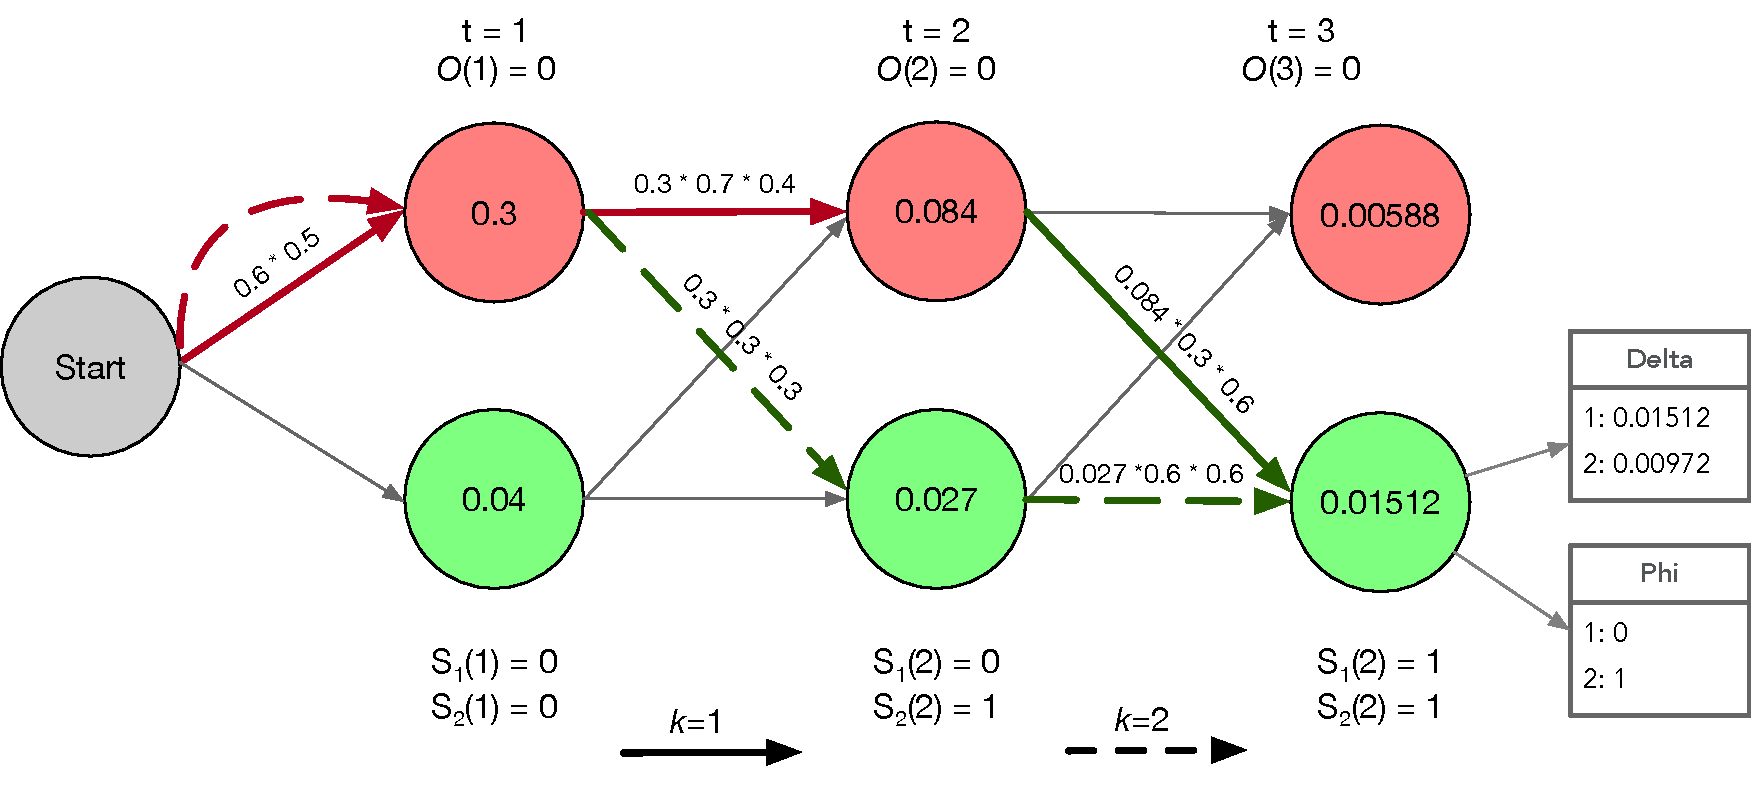
\includegraphics[width=1.0\textwidth]{ch05_pyconcat/figures/parallel_viterbi.pdf}
	\end{center}
	\caption[Viterbi decoding of Wikipedia example using our decoder]{Viterbi decoding of Wikipedia example using the Parallel decoder. Final delta and phi matrices indicate the top \textit{k} highest scoring probabilities and the state indices that led there. As the two previous states are different we don't need to consider the ranking here. The path is the solid line through the trellis, while \textit{k}=2 is indicated by the dashed line.}
	\label{fig:viterbi_parallel}
\end{figure}

\subsubsection{Serial Decoder}

The Serial Decoder, also proposed by \cite{Seshadri1994}, differs from the Parallel decoder just implemented in that it first computes the single best state sequence using the regular Viterbi decoder, then returns the remaining $k$ one by one. Despite the less efficient connotations that the serial versus parallel labelling musters up, the authors maintain it can perform less computations as ``the $k^{th}$ best candidate is computed only when the previously found \textit{k} - 1 candidates are determined to be in `error''' \citep{Seshadri1994}.

We have not implemented the Serial decoder (yet - see \chapref{chap:conclusions} for future work!), as once again no reference code is available and its derivation is a bit harder to decipher from the paper than in the case of its parallel equivalent.

\subsubsection{\textit{k}-Shortest Paths}

We hinted that the traversal of a state space in a \acrshort{hmm} bears considerable resemblance to that of a \acrfull{dag} of vertices, edges and a set of costs to be associated with those edges. This should also be visually apparent from the trellis diagrams presented in \figref{fig:viterbi_basic} and \figref{fig:viterbi_parallel}.

Shortest path algorithms aim to solve the problem of finding the the path between two given vertices with the least cost. One of the most well-known algorithms for achieving the shortest path are those by Dijkstra or Bellman and Ford \citep{Russell2002}. Computing the \textit{k}-Shortest paths then entails returning an ordered \textit{list} of the shortest paths between the two desired vertices (from what is often called the \textit{source} to the \textit{sink}).

One of first algorithms proposed for tackling \textit{k}-Shortest path problems is known as Yen's Algorithm \citep{Yen1971}. Yen's algorithm only operates on simple or loopless graphs (like \acrshort{dag}s or trellis diagram representations of a \acrshort{hmm}) and uses a regular shortest path algorithm such as Dijkstra or Bellman-Ford in order to find the best \textit{k}=1 shortest path initially. Assuming the previous $k-1$ paths have already been found, the algorithm searches the previous path for branches that deviate with higher associated cost. It is for this reason we need to have the best initial shortest path from an existing shortest path algorithm. Thankfully many implementations exist for \textit{k} Shortest Path routing so we don't need to worry about its inner workings too greatly and can rely on its black-box functionality in many graph-based programming libraries. We avail of Yen's Algorithm in Python using the the NetworkX \cite{Hagberg2008} graph library. 

With the availability of \textit{k} shortest path routing methods and the already identified similarity between a \acrshort{hmm} trellis and \acrshort{dag} we propose here a way to reformulate a \acrshort{hmm} trellis as a \acrshort{dag} for \textit{k}-Best Viterbi decoding with \textit{k}-shortest paths. The steps taken are as follows:

\begin{enumerate}
  \item A Hidden Markov Model can be considered as a weighted directed acyclic graph or trellis graph. For a series of $T$ discrete observations and $n$ hidden states, the graph contains $n*T$ nodes and $n^{2}*T$ edges connecting $n$ nodes at $t=i$ with $n$ nodes at $t=i+1$. Edge weights correspond to the joint probability of the transition cost for each pair of nodes and the emission cost of the output symbol.
  \item First create $n*T$ nodes  for step t of the trellis.
  \item Next create the necessary $n^2*T$ edges and calculate the appropriate edge weights as given by $A_{ij}*B_{j}*(O_{t})$. 
  \item Add a start node and create edges connecting to each of the nodes at $t=0$ with weights encapsulating the initial probabilities $\pi_{i}*B_{i}*(O_{1})$.
  \item Create a sink node and connect it to all the nodes at $t=T$ with a zero weighting.
  \item Before we can run the shortest path algorithm we must make one final change to address the impedance mismatch between graph-based cost minimisation and Markov probability maximisation. The edge weights need to be converted by converting to negative log-space as in  \eqnref{eq:log_cost} for a probability $p$.
  \begin{equation}
\label{eq:log_cost}
c = -log(p)
\end{equation}
  \item To recover the original probability just apply the inverse (\eqnref{eq:prob_cost})
\begin{equation}
\label{eq:prob_cost}
p = exp(-c)
\end{equation}
\end{enumerate}

Suffice it to say step 6 and 7 are not required in unit selection for concatenative synthesis since the state space is already based on cost. \figref{fig:graph_hmm} shows an autogenerated trace of the \textit{k} shortest paths, with $k=2$, applied to a graph reformulation of the Wikipedia \acrshort{hmm} example. The order of the states are reversed, so the two output sequences are actually $S_1 = (0, 0, 1)$ and $S_2 = (0, 1, 1)$ respectively.
 
\begin{figure}
	\begin{center}
		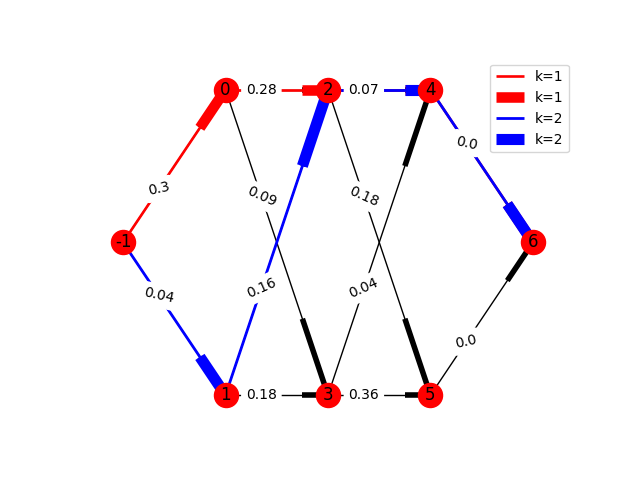
\includegraphics[width=0.65\textwidth]{ch05_pyconcat/figures/wiki_hmm.png}
	\end{center}
	\caption[Shortest Paths applied to the Wikipedia Viterbi Example]{Shortest Paths applied to the Wikipedia Viterbi Example}
	\label{fig:graph_hmm}
\end{figure}

\subsubsection{\textit{k}-Best Viterbi Decoding}

The Viterbi algorithm has proved a robust and reliable solution in many problem applications. As we emphasise in this thesis and \citep{Nuanain2017} however, it only outputs the maximum probability path from the model. This has been observed by other researchers as being restrictive when wanting to explore alternative paths through the system \citep{Schwarz2003, Brown2010}. Rabiner and Juang also observe, in the context of dynamic time warping, that the single solution Viterbi is often too sensitive and it is desirable to produce a ``multiplicity of reasonable candidate paths so that reliable decision processing can be performed" \citep{Rabiner1993}. They outline a procedure for performing \textit{k}-Best decoding using what they term the Parallel Algorithm, which can be summarised as followed.

\section{Developing a \textit{k}-Best Concatenative Synthesiser}

This chapter has hopefully presented a thorough treatise of the technical underpinnings of the key aspects of concatenative synthesis, organised by the conceptual stages of unit decomposition, analysis and unit selection, along with the presentation of two substantial contributions in the case of analysis and unit selection.

Now we turn the effort to putting all these components together to actually create some sounds. This is done in the context of PyConcat, a framework for concatenative synthesis that coalesces the previously described state of the art methods as well as novel ones like \textit{k}-Best unit selection. Some experimental evidence is also exposed that confirms the validity of our contributions. The scope of this chapter is still general to all stylistic intentions. In \chapref{chap:rhythmcat} a system is described that tailors such methods specifically for rhythm-centric dance production as stipulated in the introduction of the thesis.
 
\section{PyConcat - Python Framework for Concatenative Synthesis}

A more detailed technical introduction to the usage of PyConcat is offered in the Appendix along with example code, but this section will give a broad enough insight in order to conduct some studies. To perform a concatenative synthesis task with PyConcat the composer first requires a corpus of interesting sounds and a target sound they wish to emulate the sonic character of. They then provide parameters and issues instructions for performing the three key stages that are required\footnote{In fact, the system is sufficiently decoupled that any of these logical stages can be performed separately for their own purpose. For example the tool can be used solely for slicing sounds, or performing batch feature analysis on a library for the purposes of \acrshort{mir}.}

\subsection{Onset Detection and Segmentation}

The composer must choose the unit scale for segmenting sounds into their constituent units. The unit scales need not be the same for the target or corpus. The options we provide include

\begin{itemize}
  \item \textbf{Framewise} - slice the samples at uniform length $N$.
  \item \textbf{Framewise \acrshort{fft}} - slice the samples at uniform length $N$ and convert to the frequency domain. Overlap-add \acrshort{ifft} is performed on selected units before final concatenation.
  \item \textbf{Onset} - slice the soundfiles according to an onset detector.
  \item \textbf{Beats} - slice the soundfiles according to a beat detector.
  \item \textbf{None} - do not perform segmentation and use the entire soundfile. 
\end{itemize}

\subsection{Feature Extraction}

In order to effectively describe our audio content and produce meaningful similarity measures between constituent units both in the target sequence and the corpus of segmented units we need to choose a suitable set of descriptors. Selecting appropriate features is a trade-off between choosing the richest set capable of succinctly describing the signal, on the one hand, and the expense of storage and computational complexity, on the other. 

We expose all the features discussed in this chapter as options for analysing sounds so the composer can combine any of the following:

\begin{itemize}
\item \textbf{Temporal:} loudness, attack
\item \textbf{Spectral:} flatness, centroid
\item \textbf{Timbral:} \acrshort{bfcc}s, \acrshort{mfcc}s, \acrshort{gfcc}s
\item \textbf{Musical:} f0, \acrshort{hpcp}s
\end{itemize}

\subsection{Unit Selection}

Extracted features for the target units and corpus units and are stored in two matrices $T$ and $C$. Next the distance matrices $A = T * C$  and $E = C * C$ are calculated to avoid unnecessary computation later. Beforehand, however, it is important to perform any normalisation or standardisation and weighting of individual features as required.

A unit selection procedure is applied to return a sequence of corpus indices using:

\begin{itemize}
\item \textbf{Linear Search} - return an ordered list of the closest corpus units to each target unit.
\item \textbf{\textit{k}-D Tree} - return the approximate nearest neighbours for each target unit.
\item \textbf{Viterbi }- return the sequence with the minimised target and concatenation costs.
\item \textbf{\textit{k}-best Viterbi} - the top \textit{k} sequences with the minimised target and concatenation costs using parallel list decoding.
\item \textbf{\textit{k}-shortest Paths} - return the top \textit{k} sequences with the minimised target and concatenation costs using \textit{k} shortest paths.
\end{itemize}

\subsection{Transformation and Concatenation}

The unit selection stage returns a vector of indices of length $N$ or a matrix of $k*N$ indices  where $N$ is the number of target units and $k$ is the number of sequences from the $k$ best schemes. These indices correspond to individual sound units within our corpus. To produce the final audio representation we simply concatenate the floating point samples uniformly back to back, but there’s no reason why they can’t be overlapped and crossfaded at their boundaries for further smoothing as in \citep{Schwarz2006b}. 

Unlike other investigators we don't focus on complex post-selection transformations, but if there is a large discrepancy between the lengths of the target units and the corpus units or the pitch needs to be adjusted some time compression or pitch-shifting can be applied, which we facilitate through the a transformation stage utilising the Rubber Band Library\footnote{\url{breakfastquay.com/rubberband/}} which is also used in the systems of \cite{Davies2013} and \cite{Smith2015}.

\section{Analysis of the \textit{k}-Best Unit Selection}

In \chapref{chap:evaluation} we shall conduct a stringent and rigorous evaluation of the more fully-formed concatenative synthesis system described in \chapref{chap:rhythmcat}, which uses a type of linear search selection method coupled with a combination of timbral, spectral and loudness features. To conclude this chapter, however, we give a brief analysis of the two specialised \textit{k}-best and \textit{k} shortest selection units for comparative reference.

\subsection{Algorithm Performance}

\begin{figure}
	\begin{center}
		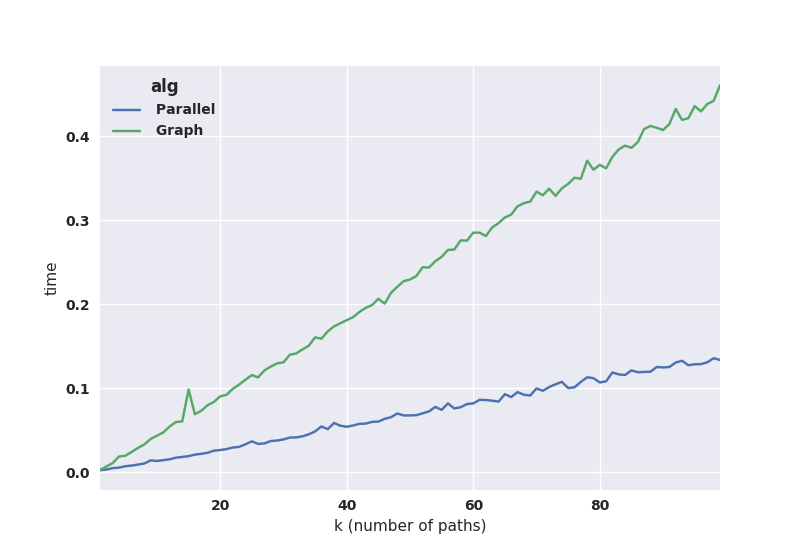
\includegraphics[width=0.9\textwidth]{ch05_pyconcat/figures/running_time.png}
	\end{center}
	\caption[Running Time Comparisons for both Algorithms]{Running Time Comparisons for both Algorithms}
	\label{fig:running_times}
\end{figure}

To compare the running times of the two implemented algorithms we took a small recording of the 8 notes of the C major scale being performing on a piano and resynthesised it with itself. \figref{fig:running_times} shows side by side of the running times for both algorithms based on the number of paths returned. Our implementation of the Parallel Decoder outperforms the NetworkX Graph approach considerably. This is mostly due the added layer of complexity of expanding the Hidden Markov Model to a fully connected directed acyclic graph. Others have noted however that NetworkX, on account of being implemented purely in Python, performs slower than other compiled graph libraries such as \textit{graph-tool} or \textit{igraph}.

It will be worth benchmarking against these implementations or reimplementing completely in C/C++. In any case, it is worth bearing in mind the real culprit in these applications: audio signal processing. The segmentation and analysis of the units took 0.926248 second for all runs.

\subsection{Equivalence and Correctness}

\begin{figure}
	\begin{center}
		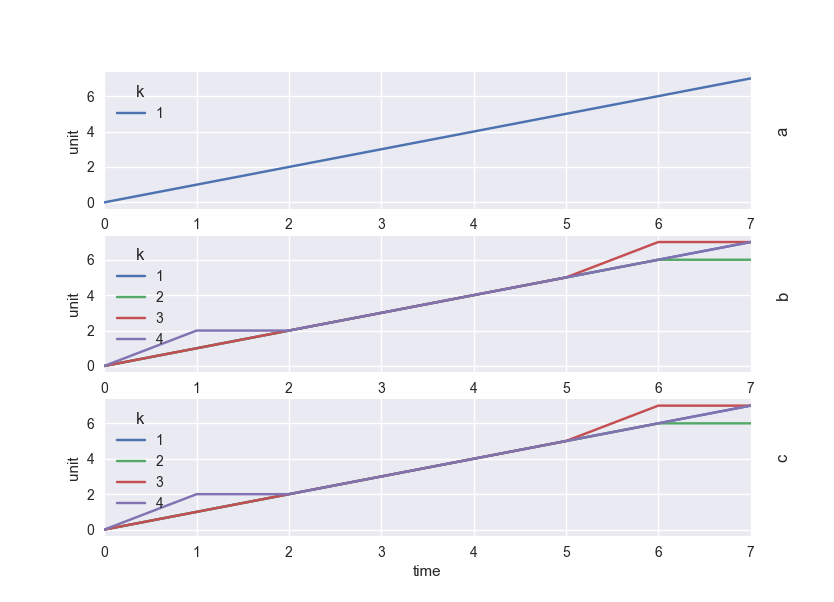
\includegraphics[width=0.9\textwidth]{ch05_pyconcat/figures/equivalence.png}
	\end{center}
	\caption[Equivalency of Unit Selection Algorithms]{Equivalency of Unit Selection Algorithms}
	\label{fig:equivalency}
\end{figure}

\figref{fig:equivalency} shows the optimal sequence generated for regular Viterbi decoding and sequences $1 \leq k \leq 5$ for the Parallel Decoder and Graph Decoder respectively. The single straight line indicates that using the chosen acoustic features and weightings, the baseline Viterbi decoder correctly reassembles its own input. The Parallel and Graph decoders both correctly return this sequence as the first optimal path also (obscured by the subsequent paths in the diagram). Looking at the other returned paths, we see very slight deviations of only one unit per path ($k$ is very small relative to the total possible paths). The possible paths, and their ordering, are identical for both algorithms.

\subsection{Pitch and Timbre Preservation}

\begin{figure}
	\begin{center}
		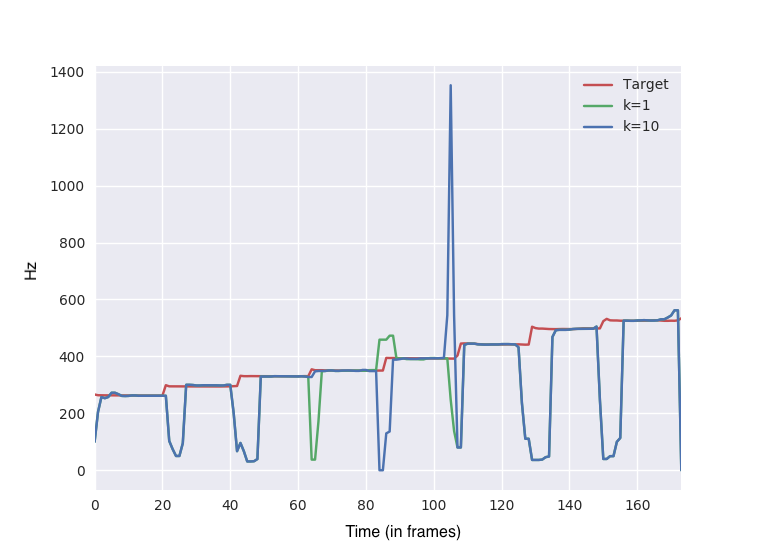
\includegraphics[width=0.9\textwidth]{ch05_pyconcat/figures/fundamental.png}
	\end{center}
	\caption[Running Time Comparisons for both Algorithms]{Running Time Comparisons for both Algorithms}
	\label{fig:fundamental}
\end{figure}

To study the \acrshort{hmm}’s acoustical output, we selected energy, fundamental frequency ($f0$) and \acrshort{mfcc} features, and chose a weighting scheme that gave preference to the $f0$ in the target cost while giving preference to the \acrshort{mfcc}s in the concatenation cost. This allows us to focus on the specific ability of the target cost in preserving the pitch between each onset in the target sample and the selected units from the corpus, while the concatenation cost attempts to preserve a continuous and coherent evolution of timbre from a variety of timbres in the corpus. We used the same piano scale sample as a target but this time using a corpus of samples from a completely different set of instruments. From a collection of orchestral samples provided freely by the London Philharmonia, 610 violin, viola, clarinet and trumpet samples were gathered with notes ranging from \acrshort{midi} A3 to G7.

\begin{figure}
	\begin{center}
		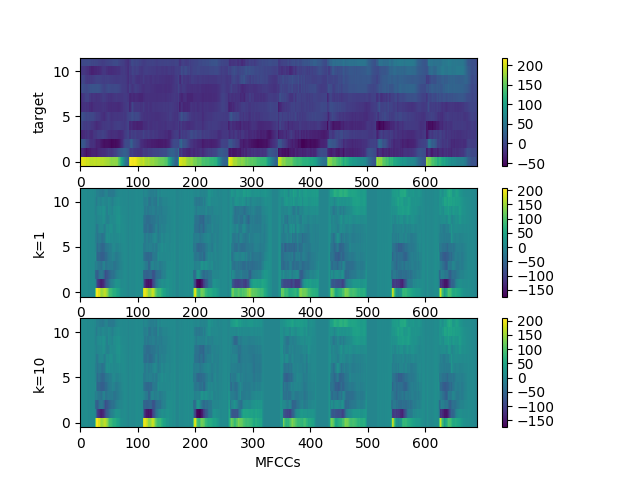
\includegraphics[width=0.9\textwidth]{ch05_pyconcat/figures/mfccs.png}
	\end{center}
	\caption[MFCC plots of k-Best Sequences]{MFCC plots of k-Best Sequences}
	\label{fig:mfcc_kbest}
\end{figure}

As we can see from \figref{fig:fundamental}, and after some median filtering to remove spurious spikes, the steady states of each pitch match for generated path 1 and generated path 10 taken as examples.

\acrshort{mfcc} plots are always a bit difficult to decipher, but while it is clear that the \acrshort{mfcc} overall profile of the target (\figref{fig:mfcc_kbest}) contrasts with the targets we can see the eight notes of the sequence reproduced and the difference in attacks that are also present in the plots of the fundamental frequencies. Again, notice lower values of $k$ produce very similar results when the size of the corpus is large, differing only by a couple of units.

